\PassOptionsToPackage{unicode=true}{hyperref} % options for packages loaded elsewhere
\PassOptionsToPackage{hyphens}{url}
%
\documentclass[12pt,]{article}
\usepackage{lmodern}
\usepackage{amssymb,amsmath}
\usepackage{ifxetex,ifluatex}
\usepackage{fixltx2e} % provides \textsubscript
\ifnum 0\ifxetex 1\fi\ifluatex 1\fi=0 % if pdftex
  \usepackage[T1]{fontenc}
  \usepackage[utf8]{inputenc}
  \usepackage{textcomp} % provides euro and other symbols
\else % if luatex or xelatex
  \usepackage{unicode-math}
  \defaultfontfeatures{Ligatures=TeX,Scale=MatchLowercase}
\fi
% use upquote if available, for straight quotes in verbatim environments
\IfFileExists{upquote.sty}{\usepackage{upquote}}{}
% use microtype if available
\IfFileExists{microtype.sty}{%
\usepackage[]{microtype}
\UseMicrotypeSet[protrusion]{basicmath} % disable protrusion for tt fonts
}{}
\IfFileExists{parskip.sty}{%
\usepackage{parskip}
}{% else
\setlength{\parindent}{0pt}
\setlength{\parskip}{6pt plus 2pt minus 1pt}
}
\usepackage{hyperref}
\hypersetup{
            pdftitle={Mortalidad en áreas menores de la Región Pampeana (2009-2011)},
            pdfborder={0 0 0},
            breaklinks=true}
\urlstyle{same}  % don't use monospace font for urls
\usepackage[margin=1in]{geometry}
\usepackage{graphicx,grffile}
\makeatletter
\def\maxwidth{\ifdim\Gin@nat@width>\linewidth\linewidth\else\Gin@nat@width\fi}
\def\maxheight{\ifdim\Gin@nat@height>\textheight\textheight\else\Gin@nat@height\fi}
\makeatother
% Scale images if necessary, so that they will not overflow the page
% margins by default, and it is still possible to overwrite the defaults
% using explicit options in \includegraphics[width, height, ...]{}
\setkeys{Gin}{width=\maxwidth,height=\maxheight,keepaspectratio}
\setlength{\emergencystretch}{3em}  % prevent overfull lines
\providecommand{\tightlist}{%
  \setlength{\itemsep}{0pt}\setlength{\parskip}{0pt}}
\setcounter{secnumdepth}{0}
% Redefines (sub)paragraphs to behave more like sections
\ifx\paragraph\undefined\else
\let\oldparagraph\paragraph
\renewcommand{\paragraph}[1]{\oldparagraph{#1}\mbox{}}
\fi
\ifx\subparagraph\undefined\else
\let\oldsubparagraph\subparagraph
\renewcommand{\subparagraph}[1]{\oldsubparagraph{#1}\mbox{}}
\fi

% set default figure placement to htbp
\makeatletter
\def\fps@figure{htbp}
\makeatother

\usepackage{booktabs}
\usepackage{longtable}
\usepackage{array}
\usepackage{multirow}
\usepackage{wrapfig}
\usepackage{float}
\usepackage{colortbl}
\usepackage{pdflscape}
\usepackage{tabu}
\usepackage{threeparttable}
\usepackage{threeparttablex}
\usepackage[normalem]{ulem}
\usepackage{makecell}
\usepackage{xcolor}

\title{Mortalidad en áreas menores de la Región Pampeana (2009-2011)}
\author{Nicolás Sacco;\footnote{Penn State,
  \href{mailto:nsacco@psu.edu}{\nolinkurl{nsacco@psu.edu}}} Iván
Williams;\footnote{Universidad Nacional de Luján,
  \href{mailto:ivanwilliams1985@gmail.com}{\nolinkurl{ivanwilliams1985@gmail.com}}}
Bernardo L. Queiroz\footnote{Cedeplar-UFMG,
  \href{mailto:lanza@cedeplar.ufmg.br}{\nolinkurl{lanza@cedeplar.ufmg.br}}}}
\date{Abril, 2020}

\begin{document}
\maketitle

\hypertarget{resumen}{%
\subsection{Resumen}\label{resumen}}

Mientras aumenta la demanada sobre estimaciones epidemiológicas para
áreas pequeñas, estudios recientes muestran una persistente brecha de
desigualdad en la esperanza de vida al nacer en América Latina. La
escasez de datos geoespaciales desafía la aplicación de diferentes
métodos para estudiar estos diferenciales de salud. En esta región, a
menudo los datos en áreas pequeñas o bien no existen, son escasos o de
muy mala calidad. Los patrones espaciales son esenciales para comprender
los resultados demográficos individuales relacionados con las
características de un lugar, también como una herramienta para la
aplicación de planes de desarrollo y para la asignación de recursos. En
base a nuevos métodos y de acuerdo con la información disponible, en
este artículo aplicamos y comparamos los resultados de tres métodos
diferentes para estimar los niveles de mortalidad en áreas pequeñas en
la Región Pampeana de Argentina, durante el período 2009-2011. Se
calculó la esperanza de vida al nacer en base a un enfoque bayesiano, un
método de tabla de vida relacional, y un enfoque demográfico indirecto,
suavizando datos espaciales de acuerdo a patrones de áreas mayores
vecinas. Las estimaciones se compararon para calcular la esperanza de
vida al nacer a partir de registros de defunción y luego se relacionaron
con áreas espaciales. Las tasas estimadas indican que existe una gran
variabilidad en la esperanza de vida al nacer y entre regiones, con una
extensión de más de seis años en la Provincia de Buenos Aires.

\hypertarget{resumo}{%
\subsection{Resumo}\label{resumo}}

À medida que a demanda por estimativas epidemiológicas para pequenas
áreas aumenta, estudos recentes mostram uma lacuna persistente na
desigualdade na expectativa de vida ao nascer na América Latina. A
escassez de dados geoespaciais desafia a aplicação de diferentes métodos
para estudar esses diferenciais de saúde. Nesta região, os dados em
pequenas áreas costumam estar ausentes, escassos ou de muito baixa
qualidade. Os padrões espaciais são essenciais para a compreensão dos
resultados demográficos individuais relacionados às características do
local, bem como uma ferramenta para implementar planos de
desenvolvimento e alocação de recursos. Com base na experiência de novas
aplicações e de acordo com as informações disponíveis, neste artigo,
aplicamos e comparamos os resultados de três métodos diferentes para
estimar os níveis de mortalidade em pequenas áreas na região de
Pampeana, na Argentina, durante o período 2009-2011. A expectativa de
vida ao nascer foi calculada com base em uma abordagem bayesiana, um
método de tabela de vida relacional e uma abordagem demográfica
indireta, suavizando os dados espaciais de acordo com os padrões das
áreas maiores vizinhas. As estimativas foram comparadas para calcular a
expectativa de vida no nascimento a partir dos registros de óbito e, em
seguida, foram relacionadas às áreas espaciais, usando análise espacial.
As taxas estimadas indicam que há grande variabilidade na expectativa de
vida ao nascer e entre regiões, com uma extensão de mais de seis anos na
província de Buenos Aires.

\hypertarget{abstract}{%
\subsection{Abstract}\label{abstract}}

As the demand for epidemiological estimates for small areas increases,
recent studies show a persistent gap in inequality in life expectancy at
birth in Latin America. The paucity of geospatial data challenges the
application of different methods to study these health differentials. In
this region, data in small areas is often either absent, scarce, or of
very poor quality. Spatial patterns are essential for understanding
individual demographic outcomes related to site characteristics, as well
as a tool for implementing development plans and for resource
allocation. Based on the experience of new applications and according to
the available information, in this article we apply and compare the
results of three different methods to estimate mortality levels in small
areas in the Pampeana Region of Argentina, during the period 2009-2011.
Life expectancy at birth was calculated based on a Bayesian approach, a
relational life table method, and an indirect demographic approach,
smoothing spatial data according to patterns of neighboring larger
areas. Estimates were compared to calculate life expectancy at birth
from death records and then related to spatial areas, using spatial
analysis. Estimated rates indicate that there is great variability in
life expectancy at birth and between regions, with an extension of more
than six years in the Province of Buenos Aires.

\begin{center}\rule{0.5\linewidth}{0.5pt}\end{center}

\hypertarget{introducciuxf3n}{%
\section{Introducción}\label{introducciuxf3n}}

¿Subsisten disparidades de mortalidad entre las áreas pequeñas?
Investigaciones demográficas previas sobre mortalidad sostienen que los
diferenciales geográficos serían gradualmente convergentes durante la
transición epidemiológica, gracias a las políticas de salud pública y
las mejoras en la calidad de vida (Borges
\protect\hyperlink{ref-Borges2017}{2017}). En la mayoría de los países
de ingresos altos y medios, la esperanza de vida al nacer (\(e_0\))
aumentó a principios del siglo XX, debido al avance del conocimiento y
la tecnología médica para combatir las enfermedades infecciosas y las
mejoras en las condiciones de vida asociadas con el desarrollo
socioeconómico.

Aunque los diferenciales socioeconómicos de mortalidad contribuyeron a
mantener la hipótesis de la desigualdad persistente en la muerte durante
y después de la transición epidemiológica, algunos autores esperan que
los resultados de salud y las disparidades se extingan a medida que se
desarrolla el cambio demográfico. Sin embargo, puntos de vista
retrospectivos muestran que los diferenciales de mortalidad son
persistentes y han aumentado con el tiempo, en muchos casos de acuerdo a
la condición socioeconómica(Borges
\protect\hyperlink{ref-Borges2018}{2018}). De todos modos, es útil tener
en cuenta si estas disparidades continúan y/o surgen independientemente
de escenarios iniciales auspiciosos.

La explicación teórica más persuasiva de estos temas argumenta que la
relación entre mortalidad y posición socioeconómica se ha mantenido a lo
largo del tiempo debido al acceso diferencial de clase social a la
tecnología de la información y a la salud (Miech
\protect\hyperlink{ref-Miech2011}{2011}). Esta hipótesis de causa-efecto
condujo a importantes desarrollos de investigación y contribuciones
teóricas. Sin embargo, identificar las relaciones basadas en estos
patrones y sus resultados demográficos presenta un serio desafío en
países donde hay pocas fuentes de datos disponibles. La investigación de
la mortalidad implica intrincadas patuas de interacciones sociales,
demográficas y ambientales. Por esa razón, la demografía espacial surgió
como una perspectiva significativa para responder preguntas demográficas
(Matthews S.A.; Parker \protect\hyperlink{ref-Matthews2013}{2013}). En
ese sentido, los patrones espaciales son esenciales para comprender los
resultados demográficos individuales relacionados con las
características de un lugar.

Dado que una planificación de salud exitosa requiere medidas de
mortalidad desagregadas que reflejen con precisión las variaciones
regionales de salud, esta falta de estimaciones confiables también tiene
un impacto negativo en las políticas públicas (Fenelon
\protect\hyperlink{ref-Fenelon2013}{2013}). Las estimaciones adecuadas
de mortalidad a nivel local también son esenciales para la
identificación de poblaciones más vulnerables, el desarrollo de
políticas sólidas de salud pública en todas las regiones y el logro de
los Objetivos de Desarrollo Sostenible (ODS).

Sobre estas cuestiones, aportes metodológicos recientes se han
desarrollado para estimaciones de mortalidad en áreas pequeñas
(Alexander, Zagheni, and Barbieri
\protect\hyperlink{ref-Alexander2017}{2017}; Schmertmann and Gonzaga
\protect\hyperlink{ref-Schmertmann2018}{2018}; Raalte, Sasson, and
Martikainen \protect\hyperlink{ref-van_Raalte1002}{2018}). En América
Latina y el Caribe, la demanda de estimaciones epidemiológicas (y de
mortalidad, específicamente) sobre heterogeneidad a nivel subnacional
está creciendo, tanto como una herramienta para la aplicación de
diferentes planes de desarrollo como para la asignación de recursos. En
los últimos años, una serie de estudios tuvo como objetivo estimar la
mortalidad a nivel local y producir análisis de tendencias y patrones
dentro de los países de la región (Schmertmann and Gonzaga
\protect\hyperlink{ref-Schmertmann2018}{2018}; Lima and Queiroz
\protect\hyperlink{ref-LimaQueiroz2014}{2014}; Peralta
\protect\hyperlink{ref-Peralta2019}{2019}).

La continua pregunta es qué tan representativos son los promedios
regionales de la variabilidad espacial. El problema principal para
abordar esta problemática, es el de tratar con fenómenos con un pequeño
número de experimentos, y en muchos casos desconocida cobertura. La
experiencia en América Latina está liderada por Brasil, donde ya existe
un desarrollo metodológico de avance sostenido (Usama Bilal
\protect\hyperlink{ref-Bilal2019}{2019}; Peralta
\protect\hyperlink{ref-Peralta2019}{2019}; C. P. Gonzaga Marcos R.;
Schmertmann \protect\hyperlink{ref-GonzagaSchmertmann2016}{2016}; Lima
and Queiroz \protect\hyperlink{ref-LimaQueiroz2014}{2014}; Freire
\protect\hyperlink{ref-FreireEtAl2015}{2015}).

Bajo este contexto, este artículo tuvo como fin estimar el nivel de
mortalidad para áreas menores de Argentina, en este caso, departamentos.
Para ello, decidimos elaborar estimaciones de mortalidad que
ejemplifiquen la relación entre el condición socioeconómica y salud,
aplicando tres métodos diferentes para estimar y luego comparar los
niveles de mortalidad en áreas pequeñas en la Región Pampeana argentina,
durante el período 2009-2011.

\hypertarget{por-quuxe9-argetina-por-quuxe9-la-regiuxf3n-pampeana}{%
\subsection{¿Por qué Argetina? ¿Por qué la región
Pampeana?}\label{por-quuxe9-argetina-por-quuxe9-la-regiuxf3n-pampeana}}

Argentina representa un claro ejemplo de un país con pocas fuentes de
datos, pero también un caso muy interesante de la transición de la
mortalidad, que a menudo no se aborda en la literatura previa (Sacco
\protect\hyperlink{ref-Sacco2016}{2016}). En comparación con otros
países latinoamericanos, el desarrollo socioeconómico temprano de
Argentina, el alto grado de urbanización y la expansión de la educación
formal influyeron en la reducción de la mortalidad que tuvo lugar antes
que en la mayoría de los otros países de la región. Esto se dio sobre
todo debido a mejoras en las condiciones de vida asociadas con el
desarrollo socioeconómico, en lugar del avance del conocimiento y la
tecnología médica para combatir las enfermedades infecciosas. Aunque
tuvo lugar más rápidamente y comenzó desde niveles más altos, la caída
de la mortalidad en Argentina puede, en ese sentido, compararse con el
patrón seguido por los países desarrollados con mayor distancia que la
mayoría del resto de América Latina (Sacco
\protect\hyperlink{ref-Sacco2016}{2016},
\protect\hyperlink{ref-SaccoBorges2018}{2018}; GERI
\protect\hyperlink{ref-GeriMoscoso2018}{2018}; Gragnolati
\protect\hyperlink{ref-Gragnolati2015}{2015}). Con el criterio de probar
cómo performan los métodos elegidos, discriminamos la región Pampena
como espacio geográfico, ya que es la región con mayor participación en
total país, que además se caracteriza por una importante hetorogeneidad
social, económica y demográfica (Otero
\protect\hyperlink{ref-Otero2012}{2012}).

Teniendo en cuenta la información disponible del último censo de
población (2010), y las estadísticas de muerte del período, el recorte
temportal remitió a la posibilidad de utilizar los datos más recientes.
A su vez, son pocos los estudios enfocados en el análisis de mortalidad
a nivel sub-nacional en Argentina. Algunos estudios abordaron la
tendencia de mortalidad infantil (Torcida, Vega, and Velázquez
\protect\hyperlink{ref-Torcida2008}{2008}) y las comunas de la Ciudad
Autónoma de Buenos Aires (Grushka
\protect\hyperlink{ref-Grushka2013}{2013}). Por ello, debido a la poca
experiencia de estudios previos que estimen mortalidad \emph{general} en
áreas menores en Argentina, se decidió aplicar tres técnicas: una basada
en la teoría bayesiana, la segunda basada en métodos relacionales de
tablas de vida pero agregando técnicas estadísticas de suavizado, y
tercero, un enfoque demográfico clásico, considerado el método por
default debido a su simplicidad. Antes de la estimación, se realizó un
procedimiento de regionalización para aprovechar la similitud espacial
entre áreas pequeñas, independientemente de su pertenencia
político-administrativa. En este sentido, solo considerando la
información de la tabla de vida, podría haber múltiples capas de
análisis de desigualdad teniendo en cuenta distintos niveles espaciales
o administrativos.

Lo que resta del artículo se divide de la siguiente forma: en la sección
Datos se retoma un análisis inicial de calidad de datos, los problemas
encontrados y las soluciones de corrección adoptadas.\footnote{El
  material complementario, código y resultados se pueden encontrar en
  \url{https://github.com/nsacco/SubnMort}.} Luego, en Metodología se
repasan las tres metodologías de suavizamiento elgidas, redefiniendo a
su vez áreas mayores por fuera de lo estrictamente administrativo, y se
describien los procedimientos de construcción de las tablas de
mortalidad. Una vez estimada la heterogeneidad entre y dentro de los
departamentos, en Resultados brevemente describimos de la relación
observada entre la heterogeneidad interna y el nivel de mortalidad a
nivel de cada provincia seleccionada.

\hypertarget{datos}{%
\section{Datos}\label{datos}}

Utilizamos los datos administrativos del registro de defunciones del
Departamento de Estadísticas e Información de Salud del Ministerio de
Salud de la Nación (DEIS), unidad oficial del gobierno a cargo de la
administración de conteos de defunciones, y las estimaciones de
población elaboradas por el Instituto Nacional de Estadísticas y censo
(INDEC) agencia gubernamental argentina responsable de la recopilación y
el procesamiento de datos estadísticos, como los censos de población.

\hypertarget{ajuste-y-correcciuxf3n}{%
\subsection{Ajuste y corrección}\label{ajuste-y-correcciuxf3n}}

Se utilizaron los microdatos de defunción para los años de registro
2009, 2010 y 2011 provistos por el Departamento de Estadísticas e
Información de Salud (DEIS) del Ministerio de Salud de la Nación. El
registro tardío en todo el país fue de 1.05\%, y dado que la idea
habitual de compensación no es uniforme entre años y áreas pequeñas, se
decidió procesar la base de datos y tomar los registros por año de
ocurrencia (ver tabla (\ref{tab:def_tardias} en el Anexo). El porcentaje
de edad desconocida fue 0.33\%, y sexo desconocido 1.01\%. Clasificando
los eventos según provincia de residencia, la información desconocida de
departamento por provincia se clasificó en \ref{tab:SinDEP}, siendo
Ciudad Autónoma de Buenos Aires la provincia en peor posición. De estas
defunciones sin departamento de residencia conocido, el 71\% se debe a
muertes que ocurrieron en departamentos adyacentes o muy cercanos a la
Ciudad Autónoma de Buenos Aires (CABA), en el Gran Buenos Aires
(aglomerado en la provincia de Buenos Aires que es vecino de CABA): Tres
de Febrero (20\%), Vicente López (15\%), La Matanza (12\%), Avellaneda
(7\%), Lanús (5\%), Morón (5\%), San Isidro (4\%) y Gral. San Martín
(3\%)\footnote{Camisa (\protect\hyperlink{ref-Camisa1964}{1964}) notó
  este sesgo hace muchos años: 10\% de los nacimientos y muertes durante
  el período 1946-1948.}. Además, debido al cambio en la definición de
las unidades administrativas en CABA, a partir de 2011 en la base de
datos no es posible matchear los tres años de riesgo que aquí se
consideran; por ambas razones se decidió dejar de lado esta
jurisdicción.

Los datos desconocidos en áreas pequeñas son un problema importante, tal
como se observa en la Tabla (\ref{tab:UnkSexAge} del Anexo). Teniendo en
cuenta solo las provincias pampeanas, Buenos Aires poseía los
departamentos con el mayor porcentaje de edad y sexo desconocidos, con
valores más elevados en sexo, siendo el líder el departamento General
Pueyrredón con 7.3\%. Debido a ello, adicionalmente no se realizó una
desagregación por sexo. Las categorías desconocidas (en variables edad,
provincia de residencia y departamento de residencia) se distribuyeron
proporcionalmente debido a su peso menor.

Para la población expuesta al riesgo de cada departamento se utilizó la
población estimada por el INDEC (Instituto Nacional de Estadística y
Censos) a mediados de año en 2010, y se aplicó la estructura observada
en el censo 2010 (INDEC \protect\hyperlink{ref-INDEC2015}{2015}). Luego,
en lugar de promediar los tres años de riesgo, se tuvo en cuenta los
años-persona en que las personas hubiesen vivido en el período de tres
años entre 2009 y 2011 y la fecha censal, siguiendo la propuesta de
Gonzaga y Schmertmann
(\protect\hyperlink{ref-Gonzaga_Schmertmann_2016}{2016}). Este
procedimiento permitió, primero, suavizar un poco la mala declaración de
edad, que podría aportar un mayor sesgo para la comparación de tasas
cuando el recuento de muertes no sigue este patrón por edad; y segundo
permitó aprovechar las correcciones de omisión hechas por INDEC en el
total\footnote{No está claro la metodología aplicada para la población
  ajustada a mitad de año en los departamentos, y si tiene en cuenta una
  corrección de ``residencia'' (INDEC
  \protect\hyperlink{ref-INDEC2015}{2015})}. Para eso se asumió una
distribución uniforme de la fecha de nacimiento dentro del año y la
población cerrada. Se utilizó una función de supervivencia única para
todos los distritos, aplicando las mismas tablas de vida estándar que
Gonzaga and Schmertmann
(\protect\hyperlink{ref-Gonzaga_Schmertmann_2016}{2016}) (una media
representativa de la Base de Datos de Human Mortality Database en años
posteriores a 1969) pero en nuestro caso ponderada por un índice de
masculinidad de 1.04 al nacer, para obtener ambos sexos\footnote{Se
  puede lograr una suavización similar, pero con menos interpretación
  demográfica, con una regresión local (procedimiento \emph{loess} en el
  software R) de 3 veces el recuento censal de población (James et al.
  \protect\hyperlink{ref-James2014}{2014}))}. La Figura
(\ref{fig:AdjExp}) muestra los ajustes realizados.

\begin{figure}

{\centering 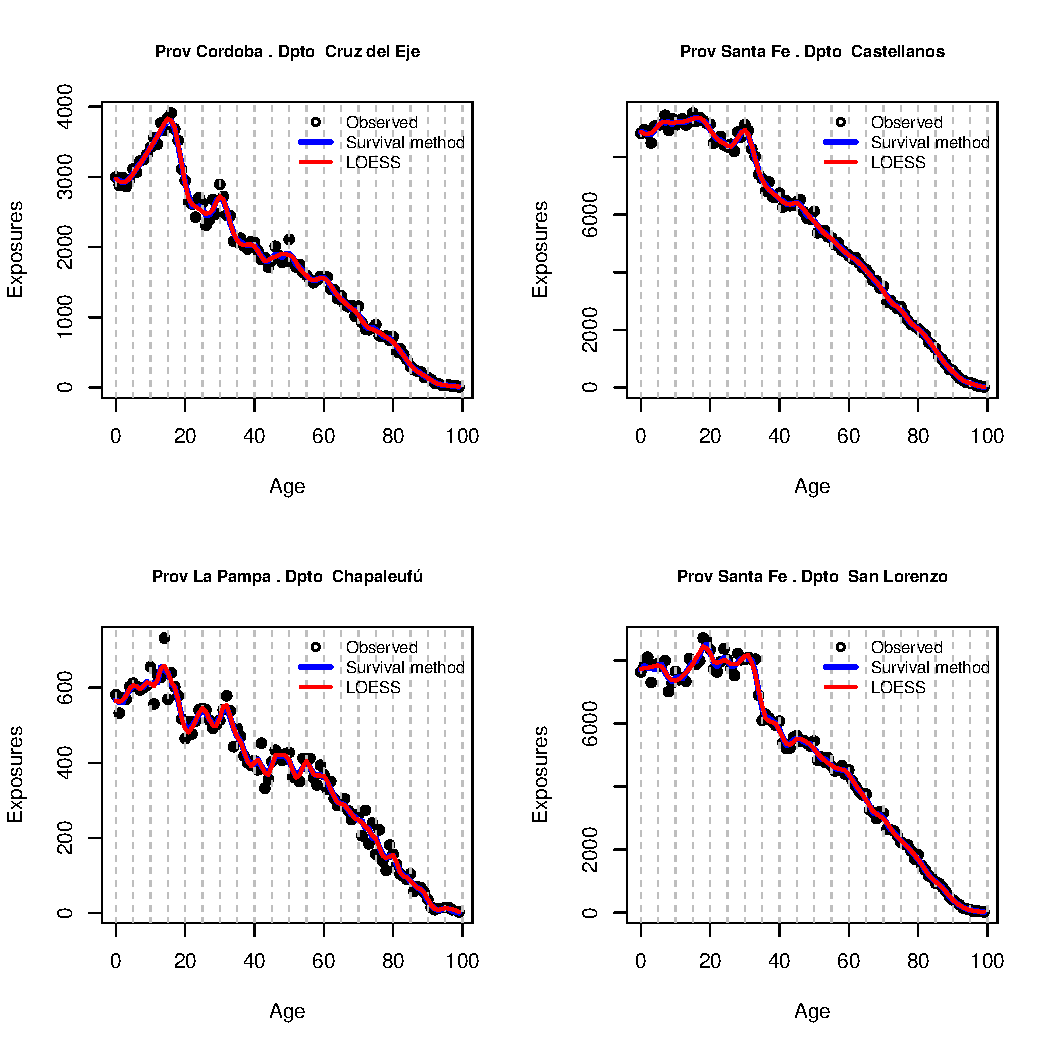
\includegraphics[width=0.7\linewidth]{/Users/nicosacco/GitHub/academicos/research/SubnMort/analysis/plots/AdjExp} 

}

\caption{Ajuste de exposición 2008-2010. Cuatro casos. Fuente: elaboración propia en base a INDEC (2013)}\label{fig:AdjExp}
\end{figure}

\hypertarget{chequeos-de-consistencia}{%
\subsection{Chequeos de consistencia}\label{chequeos-de-consistencia}}

Se conocen diversas propuestas metodológicas para abordar el problema de
cobertura de muertes en áreas menores, dependiendo de la información
auxiliar con que se cuente (Preston et al.
\protect\hyperlink{ref-Preston1980}{1980}; Bennett and Horiuchi
\protect\hyperlink{ref-Bennett_Horiuchi_1984}{1984}; Schmertmann and
Gonzaga \protect\hyperlink{ref-Schmertmann2018}{2018}; Alexander,
Zagheni, and Barbieri \protect\hyperlink{ref-Alexander2017}{2017}). La
utilización de métodos demográficos indirectos de evaluación de
cobertura es difícil de mantener en una población pequeña muy
influenciada por la migración interna debido a su baja exposición. Con
el objetivo de visualizar posibles problemas de datos de calidad en los
departamentos, se realizaron dos ejercicios.

Primero, se utilizó el método de Brass y Coale para la estimación
indirecta de la mortalidad infantil y se mapeó con la esperanza de vida
al nacer (\(q_0\)) a partir de los datos de muerte, descritos en la
sección previa (Moultrie et al. \protect\hyperlink{ref-Moultrie}{2013}).
Se trata de un método poco preciso para poblaciones pequeñas, pero puede
dar una idea sobre los problemas en las áreas mayores (problemas
relativos al numerador o denominador). En la Figura \ref{fig:PF}),
observamos los puntos no ponderados y ponderados poblacionalmente, con
el fin de otorgar mayor relevancia a la consistencia en las áreas más
pobladas, responsables del posible sesgo de suavizamiento en los
procedimientos metodológicos, que serán descritos en la siguiente
sección. Utilizando la edad promedio de la madre al nacimiento durante
2010 para cada provincia y la familia de tablas de la Organización de
Naciones Unidas (ONU) para América Latina, de acuerdo a lo observado en
el gráfico concluímos que no hay un sesgo claro en las áreas más mayores

\begin{figure}

{\centering 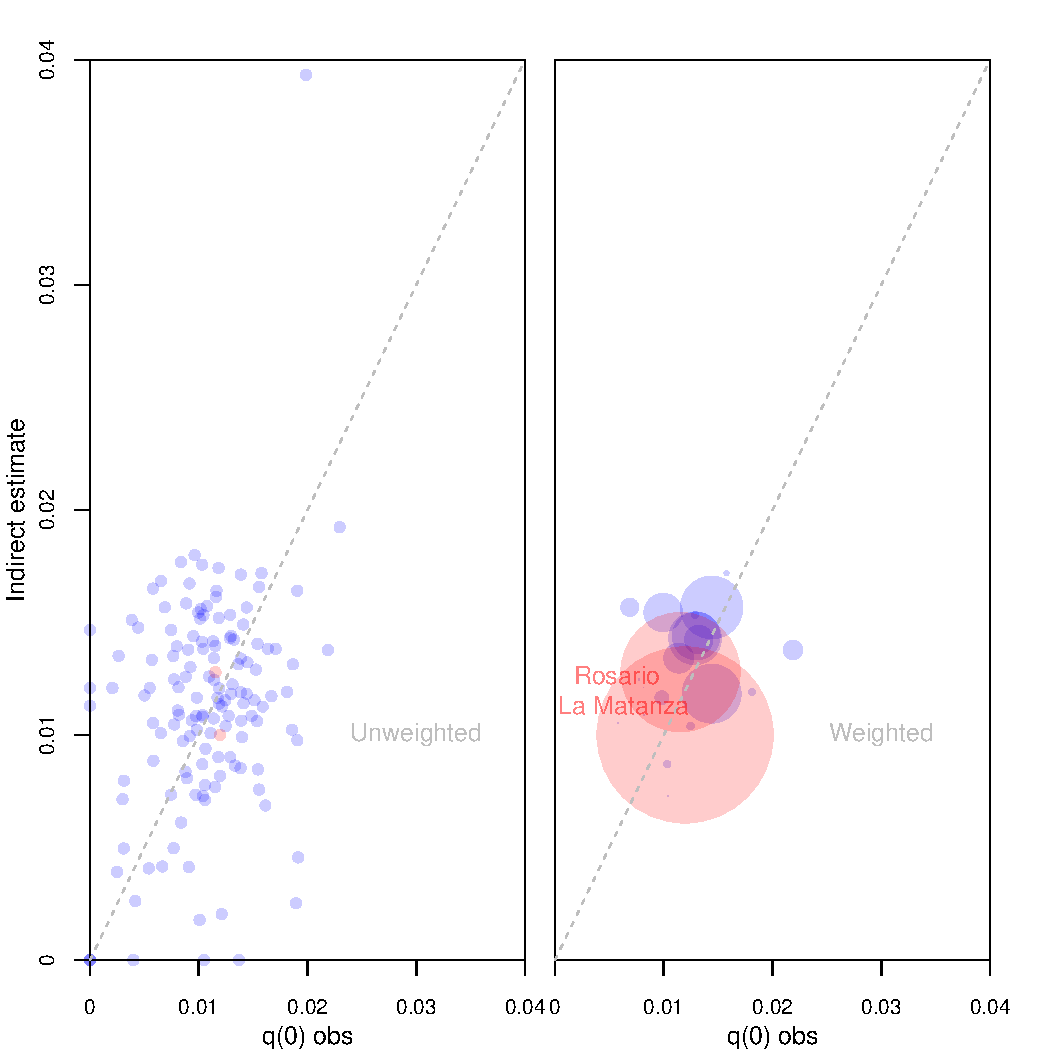
\includegraphics[width=0.7\linewidth]{/Users/nicosacco/GitHub/academicos/research/SubnMort/analysis/plots/ChekPF} 

}

\caption{Estimaciones indirectas de q(0) y tasa de mortalidad m(0) observada. Departamentos de la región Pampeana (excepto CABA). Fuente: elaboración propia en base a Cesno y estadísticas vitales.}\label{fig:PF}
\end{figure}

En segundo lugar, se mapeó cada departamento respecto al indicador
censal de pobreza Necesidades Básicas Insatisfechas (NBI) elaborado por
el INDEC y la tasa de mortalidad general estandarizada a partir de la
estructura por edad regional, buscando una relación esperada (Kaztman
\protect\hyperlink{ref-Kaztman1995}{1995}; Preston
\protect\hyperlink{ref-Preston1975}{1975}; Grushka
\protect\hyperlink{ref-Grushka2013}{2013}). En la Figura \ref{fig:NBI}
se muestran el NBI3 y el NBI4, que miden el porcentaje de hogares con
ausencia escolar de niños y la incapacidad de subsistencia (Kaztman
\protect\hyperlink{ref-Kaztman1995}{1995}). En color se destaca el
departamento más grande de la Región Pampeana, llamado La Matanza (que
contiene al 10.7\% de la provincia de Buenos Aires). Este departamento
tiene una de las tasas de mortalidad estandarizadas más bajas, pero un
índice de pobreza similar (NBI3) o mayor (NBI4) al de otros. Si bien su
desempeño en los índices de pobreza NBI1 (vivienda inconveniente), NBI2
(carencias sanitarias) y NBI3 (hacinamiento) no es tan llamativo como
los señalados, se decidió dejarlo fuera de este artículo, debido
principalmente a cuestiones metodológicas, ya que las áreas más grandes
son de extrema relevancia a la hora de suavizar las pequeñas y esto
podría sesgar los resultados.\footnote{INDEC advierte en su web sobre
  los recuentos de población por departamento en el Censo 2010, donde al
  parecer Buenos Aires fue una de las provincias con dificultades
  (\url{https://bit.ly/2R7svfX}, visitado el 10/1/2020)}

\begin{figure}

{\centering 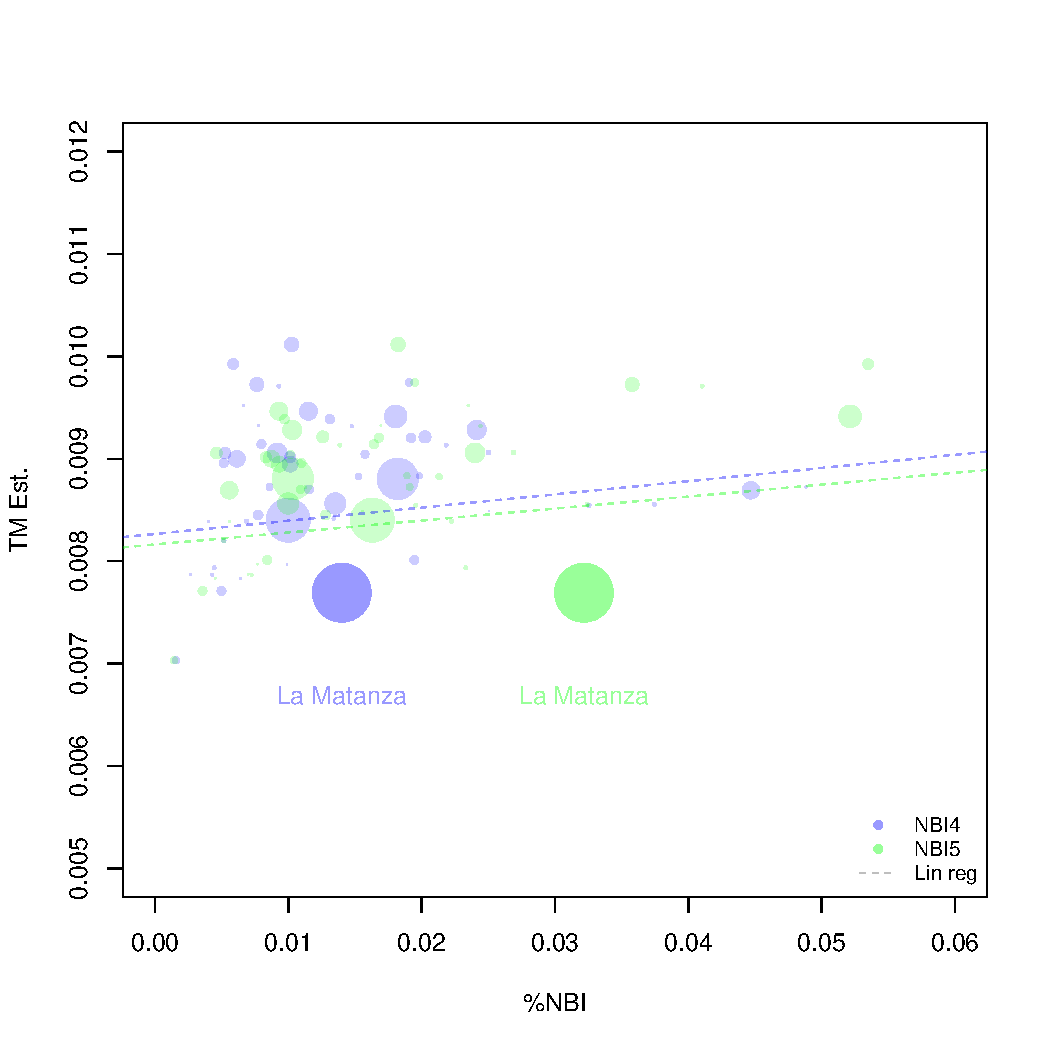
\includegraphics[width=0.7\linewidth]{/Users/nicosacco/GitHub/academicos/research/SubnMort/analysis/plots/ChekNBI} 

}

\caption{Standarized mortality rate and NBI. Departments in selected provinces. Source: own based in Census and DEIS}\label{fig:NBI}
\end{figure}

Se realizó un chequeo adicional de \(e_0\) para cada provincia a partir
de los insumos anteriores y la estimación oficial (INDEC
\protect\hyperlink{ref-INDEC2013}{2013})\footnote{A partir de lo que
  resta del artículo, se considera a Buenos Aires sin La Matanza}. Los
resultados dan una diferencia relativa (\%) de 0,002, 0.39, 0.3, 0.98,
0.34 para las provincias Buenos Aires, Córdoba, Entre Ríos, La Pampa,
Santa Fé. Por ende, consideramos aceptable nuestra aproximación dado el
año de distancia en la referencia temporal y ya que no hemos realizado
ajustes de cobertura en la defunciones, aspecto que pudo haber sido
realizado en las cifras oficiales (tabla \ref{tab:Dif_e0_INDEC}).

\hypertarget{metodologuxeda}{%
\section{Metodología}\label{metodologuxeda}}

Debido a la poca experiencia de estudios previos que estimen mortalidad
\emph{general} en áreas menores en Argentina, se decidió aplicar tres
técnicas: una basada en la teoría bayesiana, la segunda basada en
métodos relacionales de tablas de vida pero agregando técnicas
estadísticas de suavizado, y tercero, un enfoque demográfico indirecto,
considerado el método por default debido a su simplicidad. Antes de la
estimación, se realizó un procedimiento de regionalización para
aprovechar la similitud espacial entre áreas pequeñas,
independientemente de su pertenencia político-administrativa.

\hypertarget{regionalizaciuxf3n}{%
\subsubsection{Regionalización}\label{regionalizaciuxf3n}}

La definición de una región o cluster debe explorar la similitud interna
entre áreas pequeñas para poder suponer que su mortalidad es la
realización de un proceso estocástico mayor. La similitud en los
patrones de mortalidad suele abordarse por pertenecer a la misma
provincia, donde la ``distancia'' entre jurisdicciones no se mide por la
distancia geográfica o los atributos socioeconómicos (Longford
\protect\hyperlink{ref-Longford2005}{2005}).

Para ello, retomamos el enfoque propuesto por Assuncao et al.
(\protect\hyperlink{ref-AssunCao2006}{2006}), que definió áreas mayores
internamente homogéneas y con condición de contigüidad en el espacio.
Primero se realizó un gráfico de conectividad entre los centroides y
luego se calculó el \emph{costo} entre ellos (distancia euclidiana en
nuestro caso). Luego, un procedimiento de iteración estimó el árbol de
expansión mínimo, que es el árbol conectado con un costo mínimo, medido
como la suma de las diferencias en todos los bordes. Finalmente, se
realizó un procedimiento de partición cortando el borde que minimiza la
varianza dentro de los dos grupos resultantes. Debido a que probar todas
las combinaciones posibles en cada partición es un problema
computacional, los autores propusieron un enfoque heurístico. Una
sobreclusterización aumentaría la homogeneidad pero también aumentaría
la varianza en las unidades más pequeñas debido a que no hay suficientes
casos. Esa es la razón para establecer umbrales mínimos de población o
áreas menores resultantes en cada parea mayor, siendo de 20
departamentos el elegido en este caso.

Como insumos para el procedimiento de regionalización, utilizamos los
archivos \emph{shape} del INDEC disponibles en línea y el índice de NBI
del censo, ambos por departamento\footnote{\url{https://bit.ly/2sVpK9u},
  visitado el 10/01/2020.}. Se re-escaló el índice a unidades de
desviación estándar y aplicó la metodología comentada anteriormente,
implementada en el paquete \emph{spdep}, mediante la función
\emph{skater} (Bivand \protect\hyperlink{ref-Bivand2019}{2019}).

Con esta segmentación se obtuvo un aumento de 14\% en la varianza entre
grupos y una disminución no tan importante de 1\% en la varianza
promedio dentro los grupo. El nuevo clúster resultó distinto entre sus
partes y algo menos de variación relativa interna (ver Figura
\ref{fig:cluster}).

\begin{figure}

{\centering 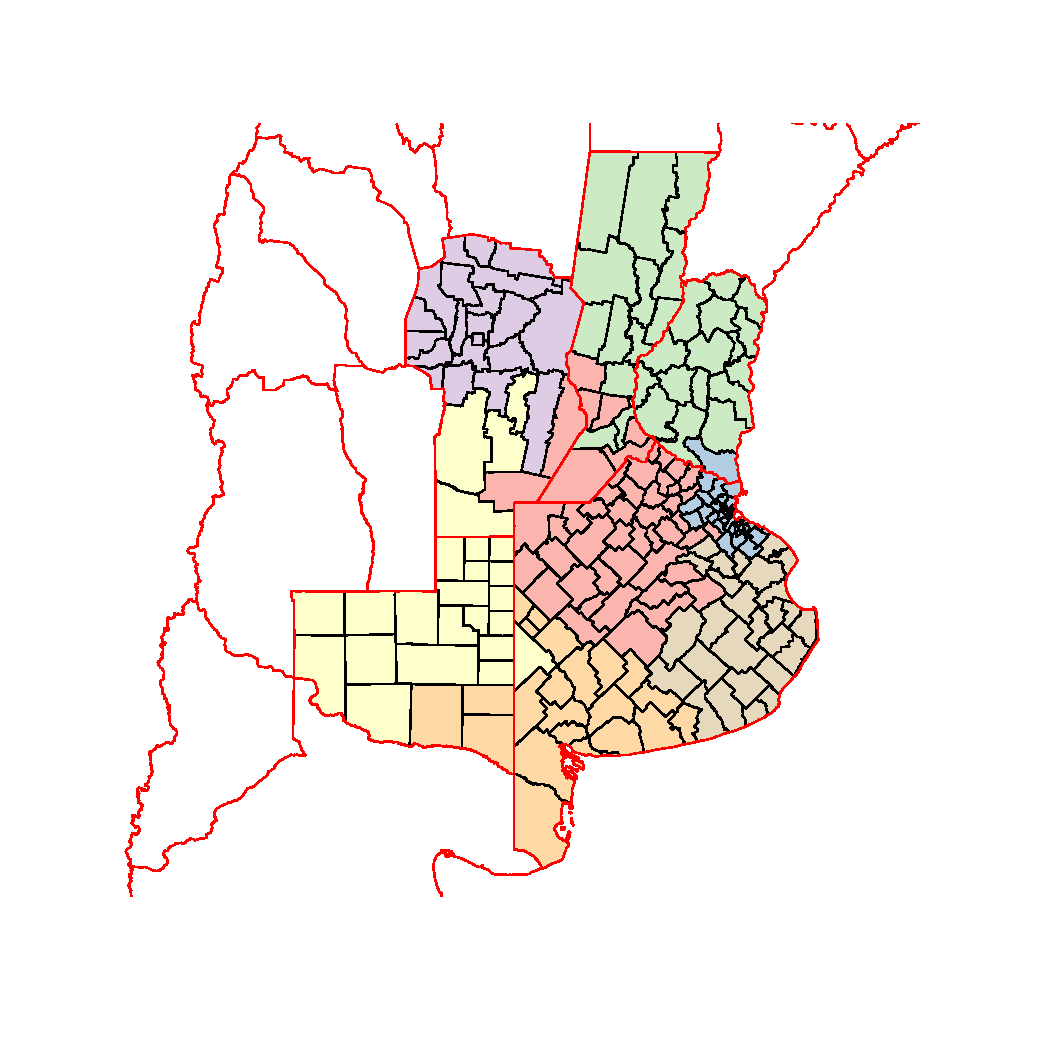
\includegraphics[width=0.7\linewidth]{/Users/nicosacco/GitHub/academicos/research/SubnMort/analysis/plots/cluster} 

}

\caption{Regionalización de departamentos. Source: Elaboración propia en base a Censo y Estadísticas Vitales}\label{fig:cluster}
\end{figure}

\hypertarget{muxe9todos-de-estimaciuxf3n}{%
\subsubsection{Métodos de
estimación}\label{muxe9todos-de-estimaciuxf3n}}

Aunque Argentina generalmente se clasifica como un país con buenas
estadísticas registrales de muerte (Jaspers and Orellana
\protect\hyperlink{ref-JaspersOrellana1994}{1994}; Luy
\protect\hyperlink{ref-Luy2010}{2010}), se conoce que hay un porcentaje
desigual de muertes infantiles no registradas por provincia (DEIS
\protect\hyperlink{ref-DEIS2016}{2016}). En este sentido, dado que la
fuente de datos es un registro, y pensando en la estimación de las tasas
de mortalidad por edad, se podría concluir que no habría varianza, y que
el sesgo (ambos componentes del error cuadrado medio de un estimador)
vendría dado por el patrón de casos omitidos en cada jurisdicción. Como
se mencionó anteriormente, este segundo componente del error no se
abordará en este trabajo debido a que no hay información sobre su
distribución por áreas pequeñas. Con respecto al primero, pese a lo
mencioando, existen fenómenos con un pequeño número de ``experimentos''
(pocos expuestos en nuestro caso), que tienen una mayor variación en sus
estimaciones, por lo que requiere un tratamiento especial para reflejar
el riesgo de mortalidad subyacente (Brillinger
\protect\hyperlink{ref-Brillinger1986}{1986}). Para lograrlo, utilizamos
y comparamos (aunque sin conclusiones finales sobre su
\emph{performance} comaparada) tres métodos diferentes, los cuales se
diferencian en la forma en que las áreas menores \emph{toman prestada}
información del área mayor que las contiene.

El método empírico bayesiano mejora la eficiencia estadística de los
estimadores de las tasas de mortalidad por edad, disminuyendo la
varianza en los casos de jurisdicciones pequeñas (Efron and Morris
\protect\hyperlink{ref-Efron1972}{1972}; Marshall
\protect\hyperlink{ref-Marshall1991}{1991}; Longford
\protect\hyperlink{ref-Longford2005}{2005}; Assunção et al.
\protect\hyperlink{ref-Assuncao2005}{2005}). La idea es que, suponiendo
que las diferentes observaciones de cada área procedan de una
distribución a \emph{priori común}, cada estimación se puede mejorar
utilizando la información de las otras. La distribución \emph{a priori}
corresponde a la distribución conjunta del vector de tasas de mortalidad
por edad del área mayor. Luego, a través del comportamiento observado en
cada área menor, se produce el ajuste bayesiano de la distribución de
mortalidad \emph{a posteriori}. La característica de ``empírico'' radica
en que las distribuciones de los parámetros del área mayor se estiman
también a partir de los datos observados, en este caso por el método de
los momentos.

En lo que respecta al caso univariable, se consideraron grupos de edad
de cinco años, ya sea en un área \(i\), bajo el supuesto que la
distribución de muertes \(d\) es un proceso de Poisson, con una media
esperada de \(E(d_ {x,4}^{i}|{m_{x,4}^{i}})=N_{x,4}^{i}m_{x,4}^{i}\),
siendo \(N\) las exposiciones y \(m\) la tasa de mortalidad.

Primero se consideró a \(\hat{m}_{x,4}^{i}=D_{x,4}^{i}/N_{x,4}^{i}\)
como el estimador de máxima probabilidad de la tasa \(m_{x,4}^{i}\) en
el área \(i\), que son \(iid\) generados a partir de \(m_{x,4}\). La
esperanza condicionada de \(\hat{m}_{x,4}^{i}\) es
\(E_{m}(E({\hat{m}}_{x,4}^{i})/m_{x,4}^{i})=E_{m}({m_{x, 4}^{i}}) = m_{x,4}\)
(tasa de área grande) y la varianza condicionada
\(V({\hat{m}}_{x,4}^{i}/m_{x,4}^{i})=\frac{m_{x,4}^{i}}{N_{x,4}^{i}}\).

La varianza total del estimador se puede expresar como la suma de la
varianza de las medias de \$ i's \$ y la esperanza de las varianzas de
\(i's\):
\(V_{m}(E(\hat{m}_{x,4}^{i}/m_{x,4}^{i}))+E_{m}(V({\hat{m}}_{x,4}^ {i}/m_{x,4}^{i}))=V_{m}(\hat{m}_{x,4}^{i})+E_{m}(\frac{{\hat{m}}}{N_{x,4}^{i}})=V_{m}(m_{x,4}^{i})+\frac{m_{x, 4}}{N_{x,4}^{i}}\).
Eso está relacionado con la relación jerárquica entre el hiperparámetro
(\(m_{x, 4}\)), los parámetros (\(m_{x,4}^{i}\)) y sus estimadores
\(\hat{m}_{x,4}^{i}\).

El estimador lineal bayesiano \(\mathring{m}_{x, 4}^{i}\) que minimiza
el error cuadrático medio de \({m}_{x,4}^{i}\) (e indicadores que son
funciones lineales de esto) es Robbins
(\protect\hyperlink{ref-Robbins1983}{1983}):

\(\mathring{m}_{x,4}^{i}=\hat{m}_{x, 4}^{i}+S_{x,4}^{i}(\bar{m}_{x,4}^{i}-\hat{m}_{x,4}^{i})\)

Nuevamente, es empírico porque \(m_{x,4}\) se estima por método de
momentos con \(\bar{m}_{x,4}\), la media ponderada de áreas pequeñas. El
factor de ``contracción'' \(S_{x, 4}^{i}\) (``shrinkage'' en la
bibliografía) es la relación entre la expectativa de la varianza
estimada en el área pequeña \(i\) y la varianza no condicionada del
estimador, que es:

\(S_{x,4}^{i}=\frac{V_{m}(m_{x,4}^{i})}{V_{m}(m_{x,4}^{i})+\frac{m_{x,4}}{N_{x,4}^{i}}}\)

Visto de otra manera, esta fórmula representa la relación entre la
varianza del área más pequeña con respecto a la suma de la varianza
total (del área más pequeña y más grande), en sintonía con un análisis
de la varianza clásica entre grupos (ANOVA). Siguiendo este
razonamiento, en un contexto de extrema homogeneidad, un área menor muy
pequeña podría caracterizarse a partir de la estimación del área más
grande (\(S_{x, 4} ^ {i} \cong 1\)). Por otro lado, las áreas de alto
peso poblacional tomarán valores cercanos a los observados
(\(S_{x,4}^{i}\cong 0\)). En el medio de estos extremos, la función
combina linealmente la estimación del área grande con respecto al área
más pequeña incluida.

Longford (\protect\hyperlink{ref-Longford1999}{1999}) extendió esta idea
a vectores de variables aleatorias (``contracción multivariada''),
estimando \(S_{x,4}^{i}\) de manera de aprovechar la correlación entre
subpoblaciones. En nuestro caso, si la tasa de mortalidad del grupo de
edad entre \(x\) y \(x+4\) del área \(i\) es mayor que el área \(j\),
una correlación alta implicaría que en edades contiguas ocurriría lo
mismo con mayor probabilidad. Si la covarianza fuera nula, este enfoque
sería equivalente al caso univariante descrito anteriormente. Los
cálculos realizados en este trabajo se realizaron para edades de 0, 1-4
y quinquenales hasta el grupo de edad abierta 80. El desarrollo se
realizó siguiendo el enfoque mostrado en Assunção et al.
(\protect\hyperlink{ref-Assuncao2005}{2005}) (páginas 543 y 544), que
estimó los parámetros por el método de momentos para las tasas de
fecundidad en Brasil.

El otro método aplicado se basó en un modelo de mortalidad relacional
llamado TOPALS (Tool for Projecting Age-Specific rates using Linear
Splines) (Beer \protect\hyperlink{ref-deBeer2011}{2011}), que utiliza un
método \emph{spline lineal} para describir los ratios entre las
probabilidades de muerte por edad de una población dada y un patrón. Una
ventaja contra el enfoque logit clásico de Brass es que TOPALS es menos
sensible al elegir el estándar. Gonzaga and Schmertmann
(\protect\hyperlink{ref-Gonzaga_Schmertmann_2016}{2016}) incluyeron esta
idea en una regresión de Poisson en las tasas de mortalidad por edad
simple, permitiendo intervalos de confianza para los resultados que
tienen en cuenta la varianza por razones de baja exposición.

Específicamente, el vector de tasas de mortalidad en el área pequeña
\(m^{i}(\alpha) = m^{*}*\exp^{\alpha B_{x}}\) es una función de los
``nodos'' spline \(\alpha\), que son las edades en las que se evaluará
el desvío respecto al patrón estándar, siendo \(m^*\) el vector de tasa
de mortalidad estándar, y \(B_{x}\) es la matriz B-spline que
multiplicada por \(\alpha\) brinda el desplazamiento lineal entre el
logaritmo de ambas tasas.

La idea es suponer que \(D_{x}\sim Poi (m_ {x} N_ {x})\) en cada área
pequeña, construir la función de probabilidad usando las muertes y
exposiciones observadas
\(\log(L(m_{x}N_{x}|D_{x}))=\sum_{\forall x}{\lbrack -m_{x}N_{x}+D_{x}\ln (m_{x})+D_{x}\ln (N_{x})-\ln (D_{x}!)\rbrack}\),
pero expresando eso en función del parámetro \(\alpha\), agregando una
penalización por distancia desde el estándar y suavizando entre edades
adyacentes. Se colocan nodos en edades más determinantes en el perfil de
mrotalidad, para luego minimizar el log-likelihood:
\(Q(\alpha )=\sum_{\forall x}{\lbrack -m(\alpha )_{x}N_{x}+D_{x}\ln(m(\alpha )_{x})\rbrack }-\sum_{k=0}^{5}{(\alpha _{k}-\alpha _{k+1})^{2}}\).

El método empírico bayesiano es particularmente apropiado en casos con
pequeñas muestras locales, variaciones regionales relevantes, y
correlaciones entre los componentes y relaciones espaciales (Assunção et
al. \protect\hyperlink{ref-Assuncao2005}{2005}). En el caso de la
regresión TOPALS, la aplicación es más una técnica de suavización que un
modelo de variabilidad espacial, por lo que se necesitan menos supuestos
sobre las relaciones entre áreas.

Finalmente, se aplicó el método de estandarización indirecta, quizás uno
de los primeros enfoques propuesta para aboradar estos problemas
(Arriaga \protect\hyperlink{ref-Arriaga2011}{2011}). Se basa en cambiar
solo el nivel del área principal para replicar las muertes del área
menor que se está estimando. Es el caso en el que no se tiene en cuenta
ninguna información sobre la forma de la mortalidad por edad del área
menor.

\hypertarget{resultados}{%
\section{Resultados}\label{resultados}}

Las estimaciones se calcularon para grupos quinquenales de edad (excepto
el primer grupo, separado en 0 y 1-4) con 90 y más como grupo abierto
final, en todos los departamentos de la Región Pampeana (excepto La
Matanza y aquellos en CABA, por motivos ya expuestos). El método TOPALS
fue pensado para aplicar en edades simples, pero en este caso, debido a
que no se corrigió la omisión en áreas pequeñas y para ser comparable
con los demás métodos, se aplicó a edades quinquenales tomando nodos en
los grupos 0, 5-9, 20-24, 40-44 y 60-64. En la Figura \ref{fig:Ajuste}
se muestran cuatro ejemplos de ajuste.

\begin{figure}

{\centering 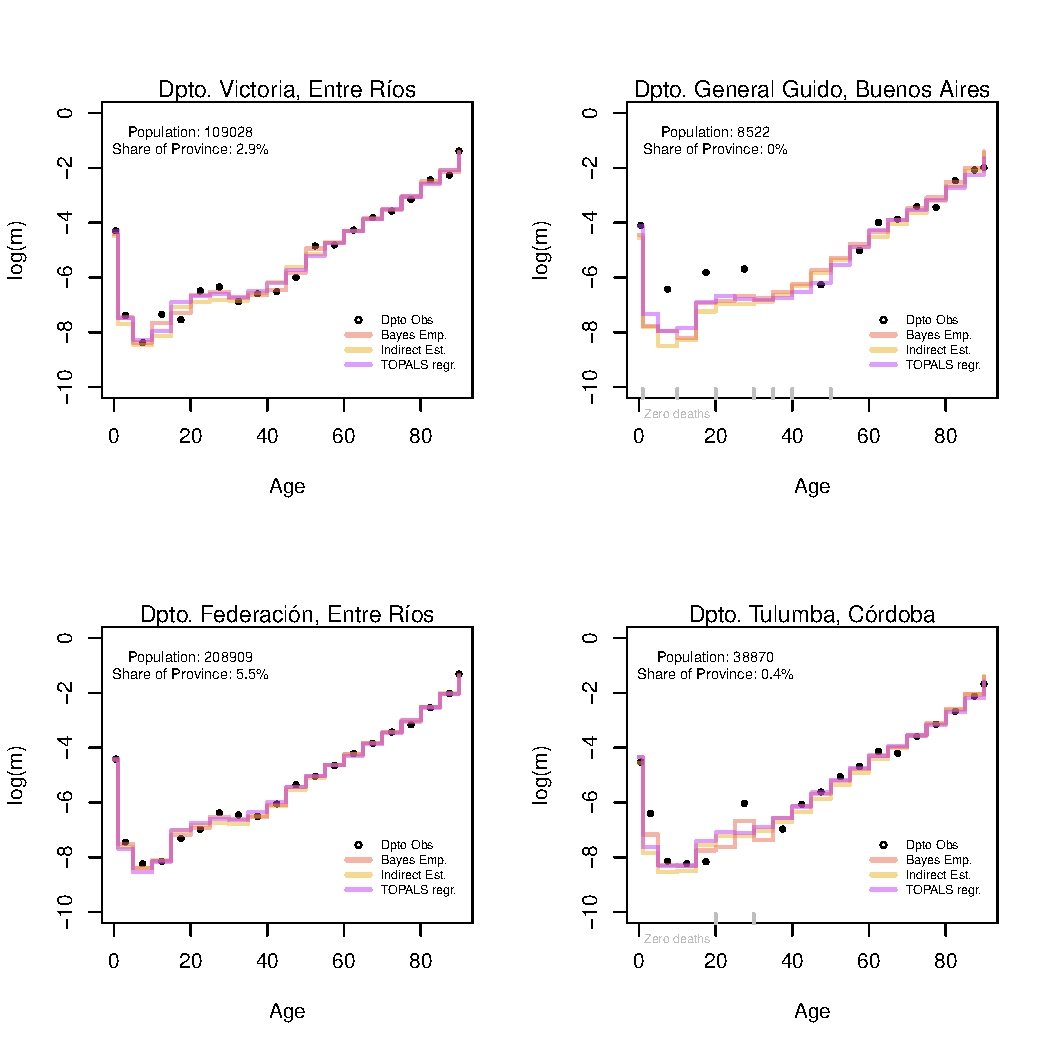
\includegraphics[width=0.7\linewidth]{/Users/nicosacco/GitHub/academicos/research/SubnMort/analysis/plots/Ajuste} 

}

\caption{Estimación de la mortalidad por Departamentos según métodos. Fuente: elaboración propia}\label{fig:Ajuste}
\end{figure}

La \(e_0\) es la medida resumen de la mortalidad para comparar niveles,
teniendo en cuenta también que el efecto de los problemas en la edad
adulta (de mayor incertidumbre en áreas pequeñas) tienen poco efecto en
las estimaciones sobre \(e_0\) en poblaciones donde la mortalidad
infantil y juvenil aún tienen un peso importante en el
indicador.\footnote{En términos matemáticos,
  \(\frac{de_0} {d \ mu_ {80 +}} = f (T_ {80 +})\) están cerca de cero
  dependiendo de la no rectangularidad de \(l_x\) y la corrección o
  cambio en la tasa. En otros términos, un cambio en estas tasas, por
  ejemplo debido a la corrección de sesgo, se pondera con
  \(l_{80}\):\(\frac{de_0} {d \epsilon} = \int_{o}^{\inf}{\frac{d\mu_x} {d \epsilon} e_x l_x dx}\)
  (Wrycza and Baudisch \protect\hyperlink{ref-Wrycza2012}{2012}).}

La correlación entre los métodos es clara: existe una gran similitud
entre TOPALS y la estimación indirecta (0.97), pero menor en Bayes
Empírico contra la estimación indirecta (1) y TOPALS (1) (Figura
\ref{fig:comparativeMeth}).

\begin{figure}

{\centering 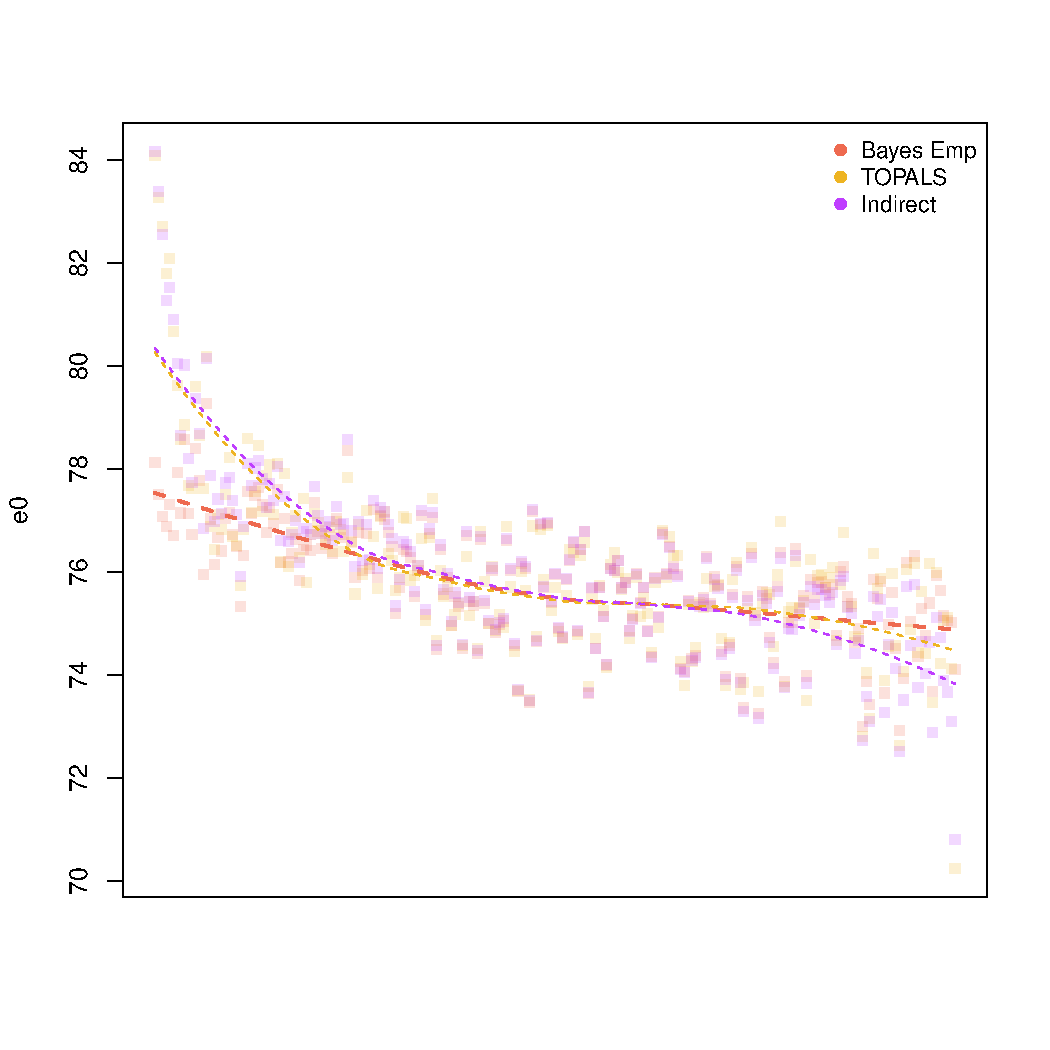
\includegraphics[width=0.7\linewidth]{/Users/nicosacco/GitHub/academicos/research/SubnMort/analysis/plots/CompMethods} 

}

\caption{Estimaciones de esperanza de vida al nacer según tres metodologías. Source: elaboración propia}\label{fig:comparativeMeth}
\end{figure}

Las principales diferencias se deben a que el método bayesiano tiende a
tomar \emph{siempre} alguna información sobre el patrón de edad,
suponiendo una correlación entre edades contiguas dado el comportamiento
global del área mayor. En los dos restantes métodos, el patrón stándard
es de mayor fuerza gravitatoria. Los departamentos donde se reportan las
mayores diferencias son aquellos con pocas celdas distintas de cero (ver
Tabla \ref{fig:Feos}).

\begin{figure}

{\centering 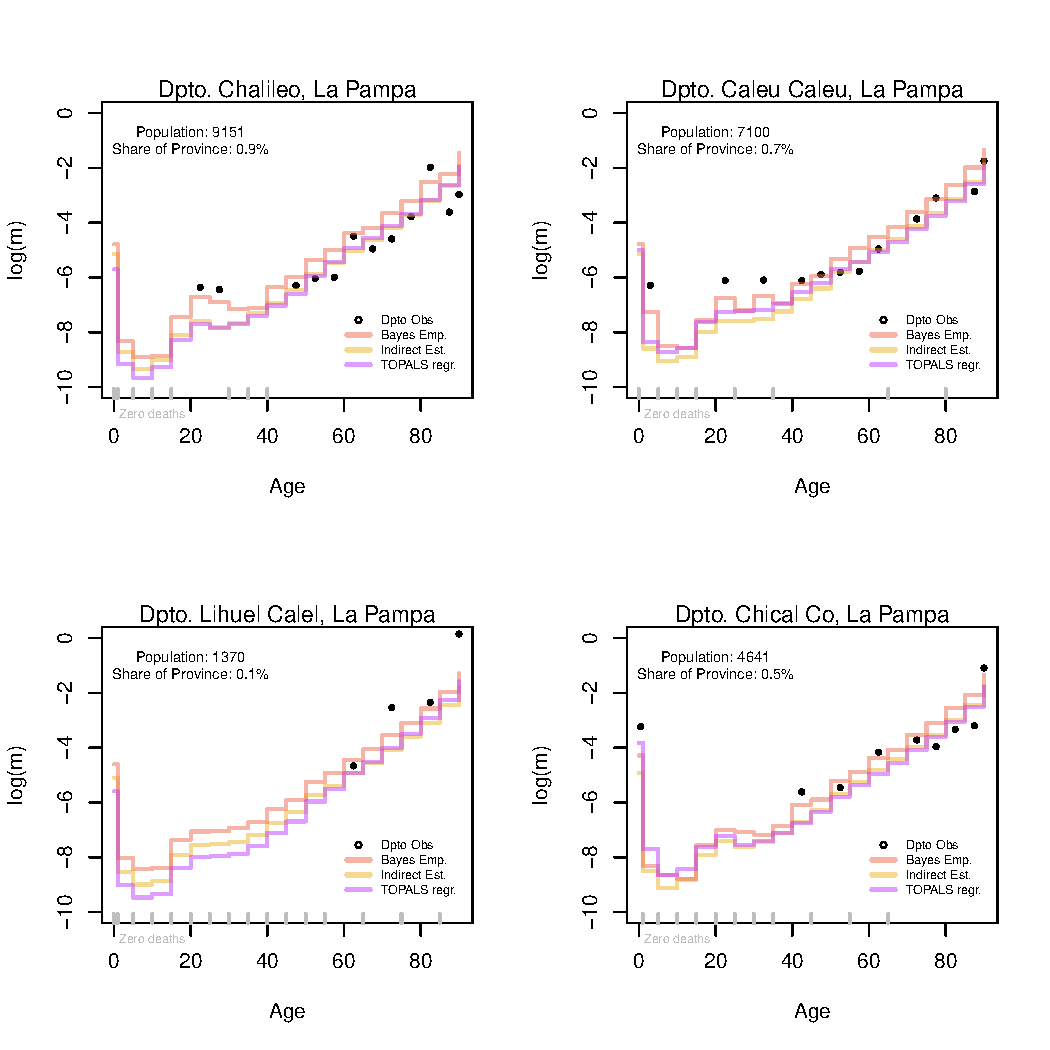
\includegraphics[width=0.7\linewidth]{/Users/nicosacco/GitHub/academicos/research/SubnMort/analysis/plots/AjusteFeos} 

}

\caption{Estimaciones de mortalidad de los departamentos con mayores diferencias entre métodos. Fuente: elaboración porpia}\label{fig:Feos}
\end{figure}

Por otro lado, se siguió el procedimiento empleado por Gonzaga and
Schmertmann (\protect\hyperlink{ref-Gonzaga_Schmertmann_2016}{2016}),
relacionando las defunciones del área mayor con las obtenidas mediante
la agregación de las estimaciones para las áreas menores (Figura
\ref{fig:consistAM}). Si bien los promedios son para los métodos
Indirecto, Bayesiano y Topals, se destaca un poco más de variabilidad en
el segundo y tercero, y un patrón singular en el primero que sugiere un
sesgo específico.

\begin{figure}

{\centering 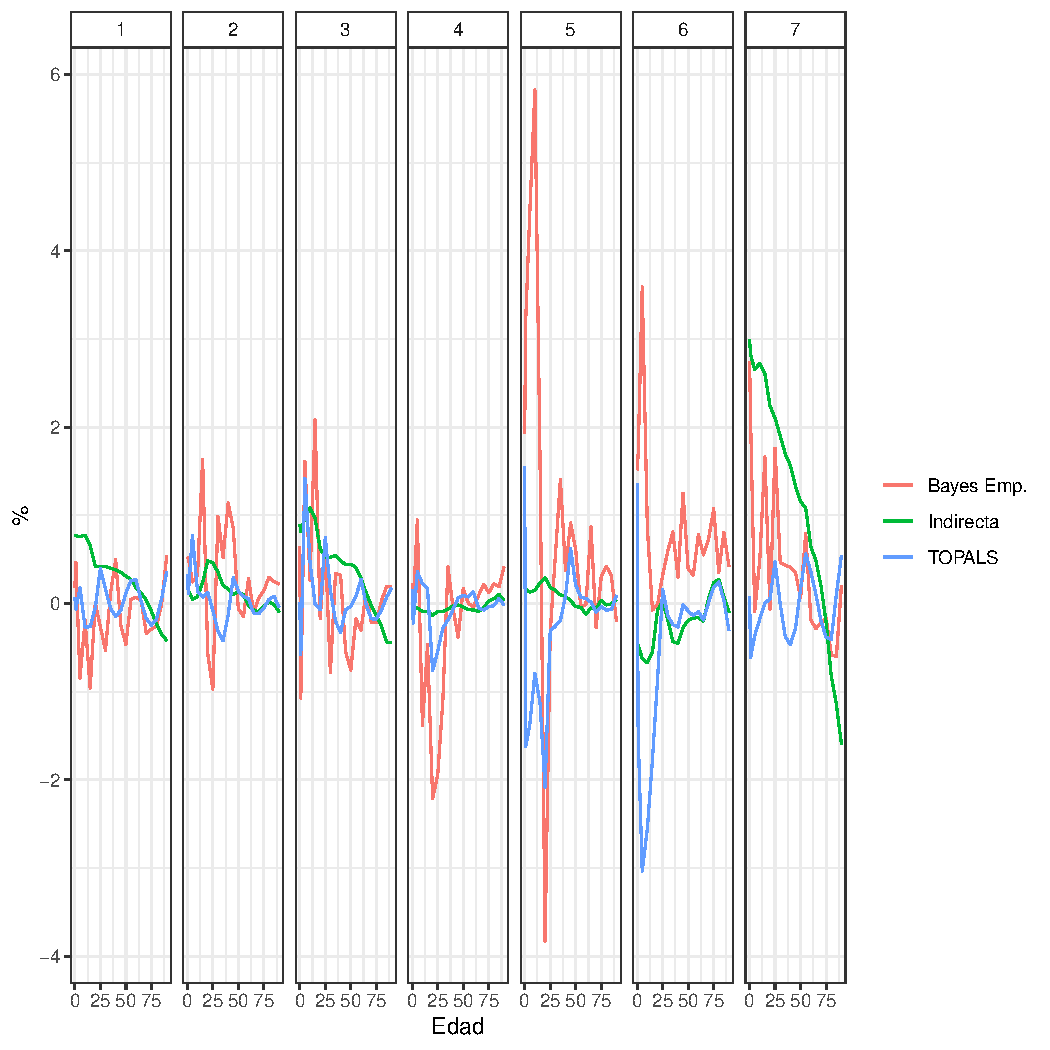
\includegraphics[width=0.7\linewidth]{/Users/nicosacco/GitHub/academicos/research/SubnMort/analysis/plots/ConsistAM} 

}

\caption{Diferencias relativas en la cantidad de defunciones por edad del área mayor. Fuente: elaboración porpia}\label{fig:consistAM}
\end{figure}

En la Figura \ref{fig:jerarq} se consideraron los resultados del método
de Bayes Empírico debido a presentar un escenario más conservador en el
rango de estimaciones (futuras líneas de investigación deberían utilizar
técncias de simulación para llegar a conclusiones más sólidas, como se
menciona al final del trabajo). Para tener en cuenta la aleatoriedad, se
realizó un proceso bootstrap de los recuentos de muertes a partir de una
distribución de Poisson del conteo de defunciones en cada grupo etario.
Esto permitió contar percentiles de las funciones de la tabla de vida y
específicamente de la esperanza de vida al nacer (ver Tablas
\ref{fig:jerarq} y \ref{tab:table_e0}, donde se muestran las
estimaciones en el intervalo 95\%).

\begin{figure}

{\centering 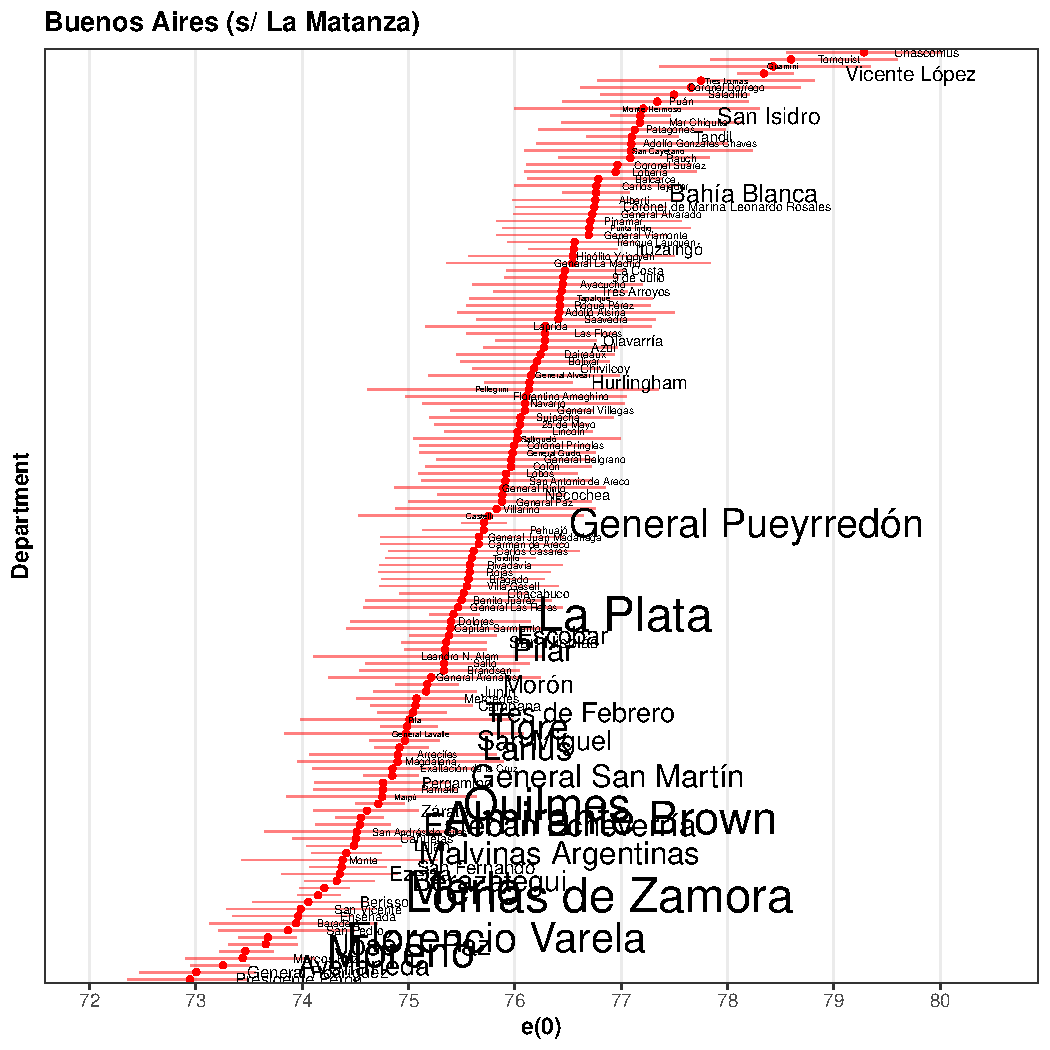
\includegraphics[width=0.48\linewidth]{/Users/nicosacco/GitHub/academicos/research/SubnMort/analysis/plots/BA} \includegraphics[width=0.48\linewidth]{/Users/nicosacco/GitHub/academicos/research/SubnMort/analysis/plots/Córdoba} 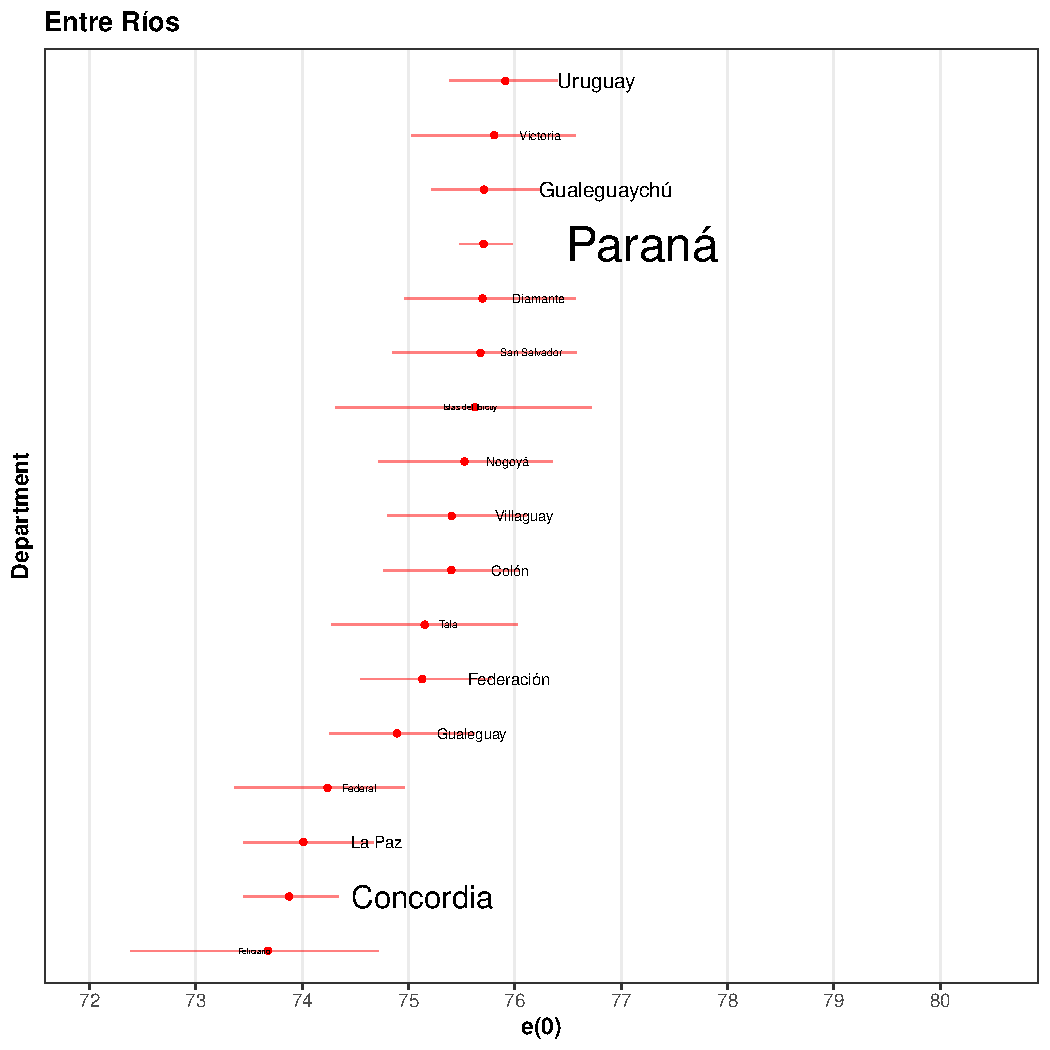
\includegraphics[width=0.48\linewidth]{/Users/nicosacco/GitHub/academicos/research/SubnMort/analysis/plots/ER} 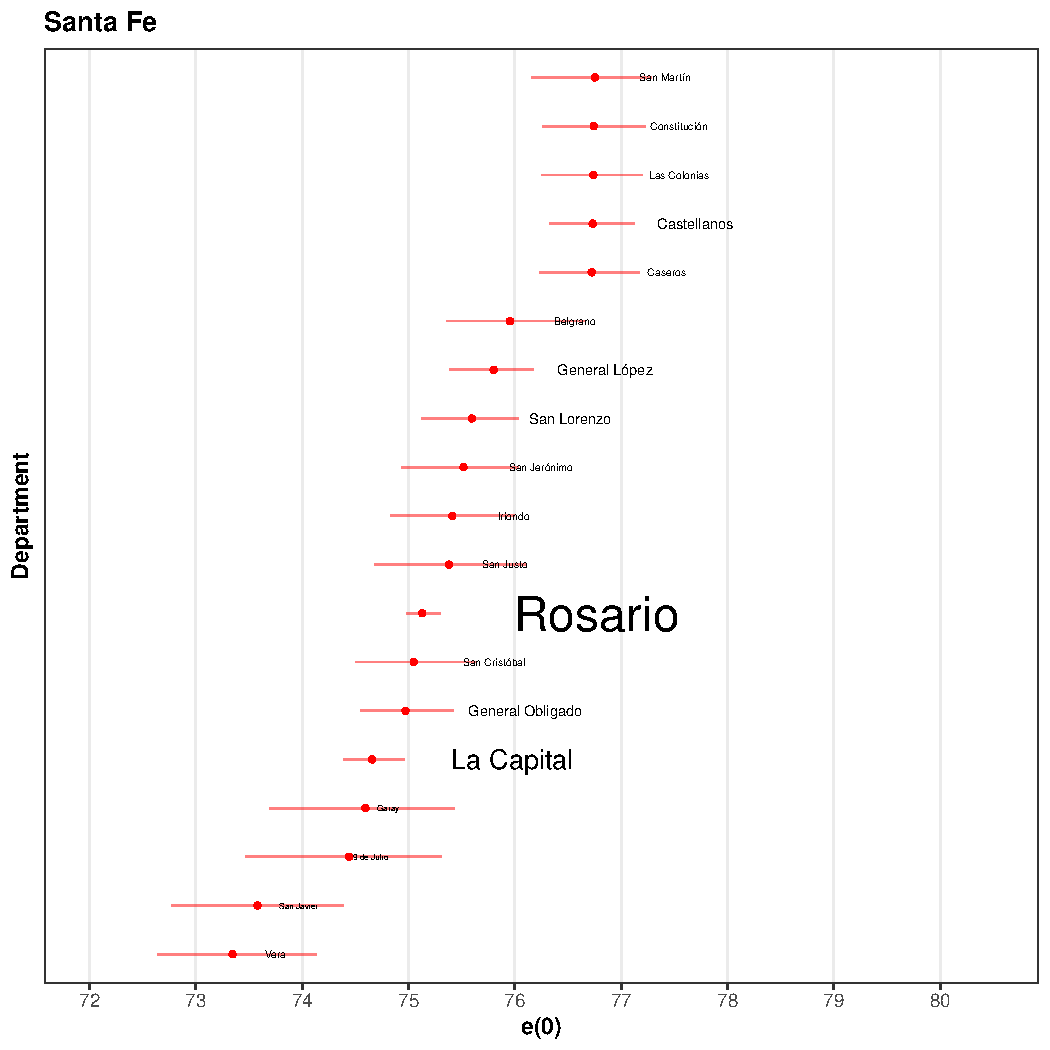
\includegraphics[width=0.48\linewidth]{/Users/nicosacco/GitHub/academicos/research/SubnMort/analysis/plots/Santa_Fe} 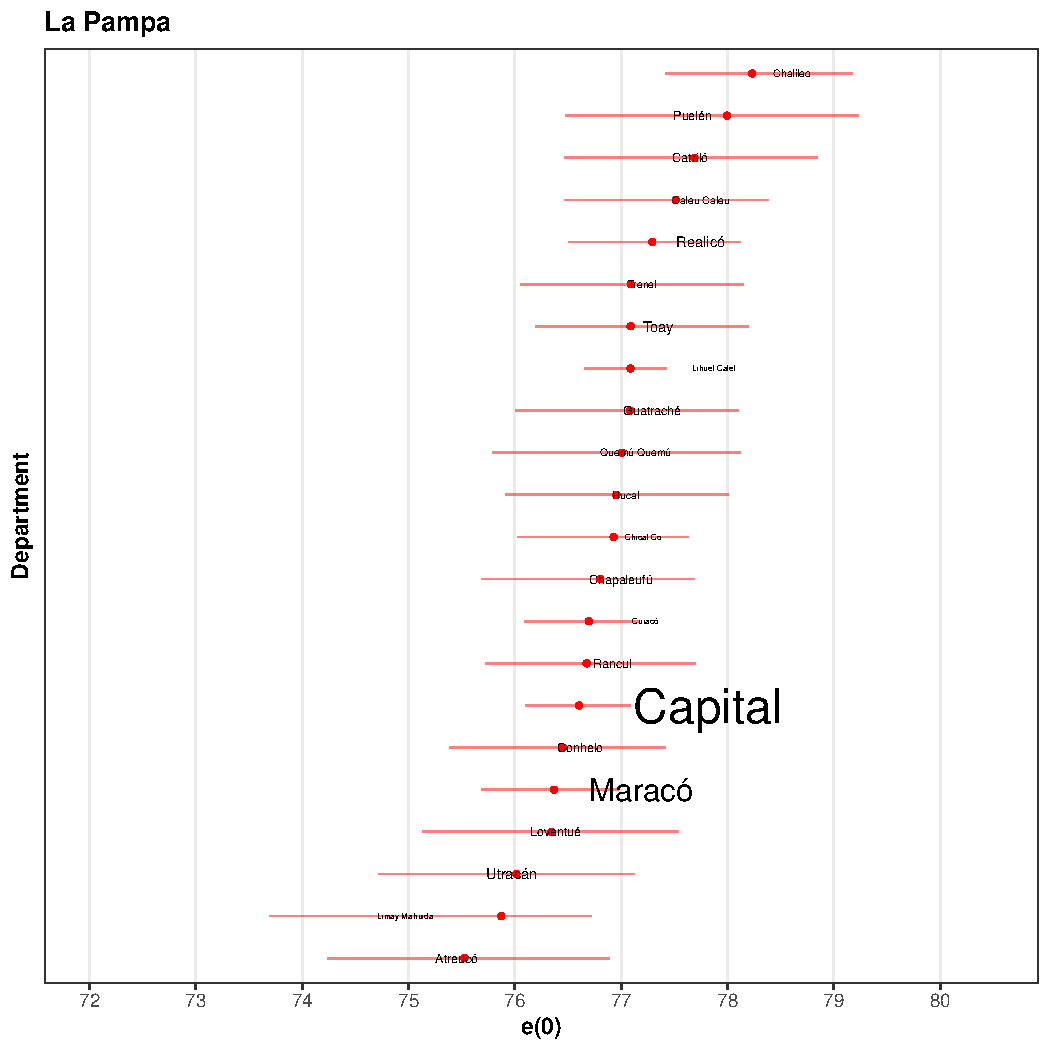
\includegraphics[width=0.48\linewidth]{/Users/nicosacco/GitHub/academicos/research/SubnMort/analysis/plots/La_Pampa} 

}

\caption{Esperanza de vida al nacer para las provincias pampeanas (excepto CABA, y Buenos Aires sin La Matanza). Ordenado según la media y con intervalos de confianza. El tamaño de los nombres sigue al tamaño relativo de la población en esa provincia. Fuente: elaboración propia}\label{fig:jerarq}
\end{figure}

\begin{table}

\caption{\label{tab:dispersion}Resumen de estimaciones por provincia. Esperanza de vida al nacer}
\centering
\begin{tabular}[t]{l|r|r|r|r}
\hline
Provincia & Promedio & n & Varianza & Rango\\
\hline
Buenos Aires & 75.7 & 133 & 1.4 & 6.3\\
\hline
Córdoba & 76.1 & 26 & 0.6 & 3.5\\
\hline
Entre Ríos & 75.1 & 17 & 0.5 & 2.2\\
\hline
La Pampa & 76.9 & 22 & 0.4 & 2.7\\
\hline
Santa Fé & 75.4 & 19 & 1.1 & 3.4\\
\hline
\multicolumn{5}{l}{\textsuperscript{a} El promedio y varianza no están ponderados}\\
\multicolumn{5}{l}{\textsuperscript{b} Fuente: elaboración propia}\\
\end{tabular}
\end{table}

Buenos Aires posee mayor cantidad de departamentos y a la vez una mayor
dispersión, medida por el rango (distancia entre máximo y mínimo) y la
varianza de los promedios (no ponderada). Conocida es su particular
división entre los partidos del Gran Buenos Aires, que forman parte del
aglomerado urbano más grande del país con la Ciudad Autónoma de Buenos
Aires, y el resto de la provincia.

\hypertarget{la-provincia-de-buenos-aires}{%
\subsubsection{La provincia de Buenos
Aires}\label{la-provincia-de-buenos-aires}}

¿Qué nos permiten decir las estimaciones? Buenos Aires es la provincia
más poblada de Argentina, conteniendo 134 áreas administrativas. En la
Figura previa \ref{fig:dispersion} se mostró su gran heterogeneidad, con
un rango estimado de esperanza de vida al ncaer de más de 6 años. La
provincia se puede dividir entre el área del Gran Buenos Aires compuesta
por 24 departamentos (área urbana que rodea a CABA) y el resto de la
superficie. Para inspeccionar el significado de los resultados, en la
Figura \ref{fig:dptosBsAs} describimos tres jurisdicciones con
exposición significativa y ubicadas a lo largo de la distribución: San
Isidro, General Pueyrredón y Moreno.

\begin{figure}

{\centering 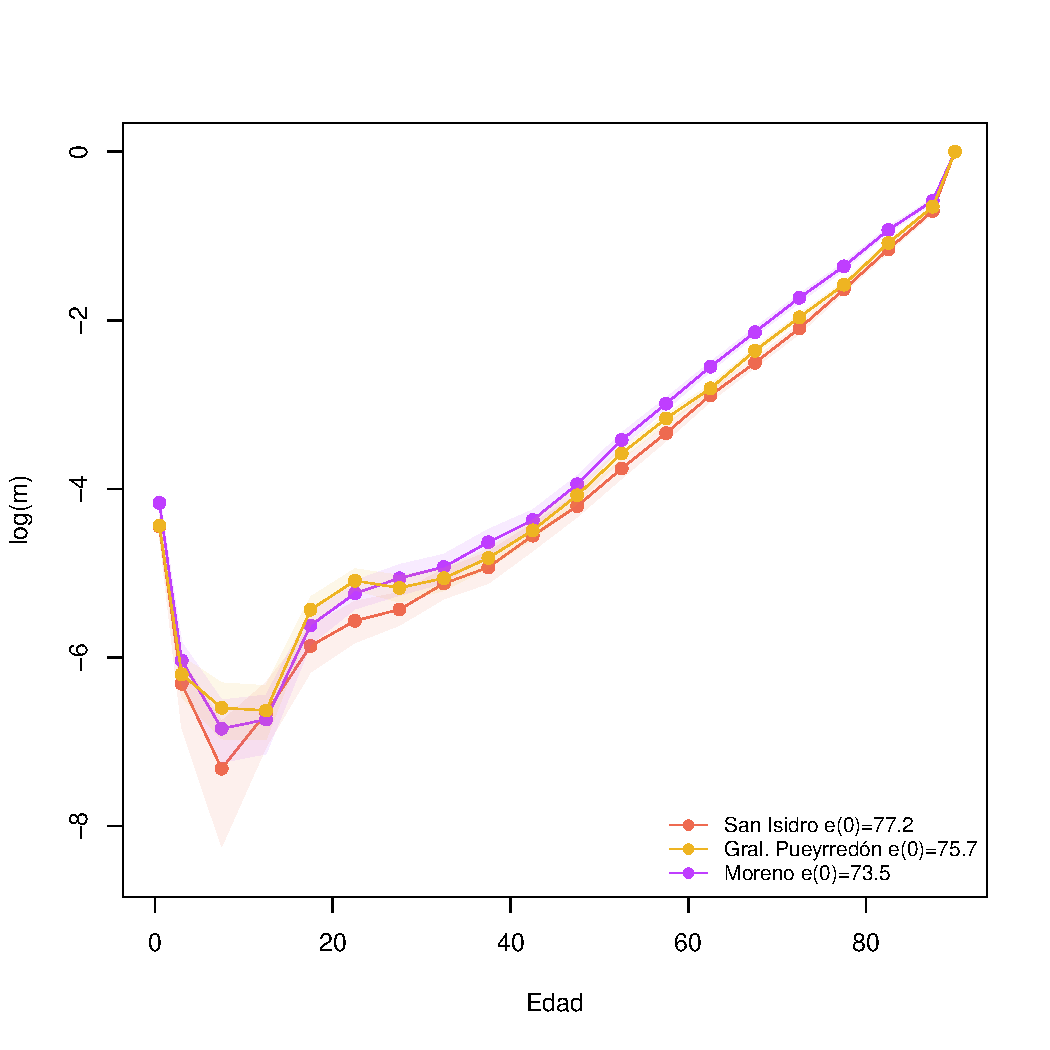
\includegraphics[width=0.48\linewidth]{/Users/nicosacco/GitHub/academicos/research/SubnMort/analysis/plots/SanIsyMoreno} 

}

\caption{Tasas de mortalidad según áreas seleccionadas de la Provincia de Buenos Aires. Fuente: elaboración propia}\label{fig:dptosBsAs}
\end{figure}

Si comparamos la mediana de las tasas por edad, Moreno presenta una
mayor mortalidad infantil pero también un mayor riesgo en adultos
mayores. \emph{A priori}, no hay ninguna razón para creer en una
exposición con omisión diferencial en mayores de 40 años de edad, por lo
que probablemente este sea un patrón de mortalidad a tener en cuenta. En
el caso de San Isidro, con la mayor esperanza de vida al nacer de este
grupo, presentó la curva más baja en el rango de edad típico de causas
externas. Finalmente, Gral. Pueyrredón tuvo la peor posición en el rango
de edad de 5 a 25 años, edades con un porcentaje importante de
mortalidad por causas prevenibles. En términos estadísticos, dado el
modelo empleado, los rangos de edad donde se pueden ensayar
comparaciones jerárquicas entre las tres jurisdicciones tomadas son
aquellos donde lás áreas no se solapan: infantil y adulta mayor a 45, y
15-24 entre San Isidro y Gral. Pueyrredón.

\hypertarget{limitaciones-y-trabajo-futuro}{%
\subsection{Limitaciones y Trabajo
futuro}\label{limitaciones-y-trabajo-futuro}}

Una de las limitaciones de esta propuesta es que se desconoce el nivel
de cobertura de las áreas menores. Se realizó un análisis de datos
desconocidos en el registro de defunciones y algunas comprobaciones
visuales sobre la consistencia entre un indicador censal socioeconómico
(NBI) y estimaciones indirectas de mortalidad infantil con el fin de
detectar posibles anomalías, pero solo enfocándose en los departamentos
de gran volumen debido a las propiedades estadísticas de los métodos. El
costo fue grande: se dejó fuera de la estimación al departamento más
grande del país, a la Ciudad Autónoma de Buenos Aires, y no se desagregó
por sexo el ejercicio. Correcciones sobre los datos deben realizarse a
partir de información externa si se deciden incorporar en futuras
investigaciones, al menos en el período considerado.

En investigaciones ulteriores, otras análisis serán necesarios. Para
realizar una comapración metodológica robusta podrían simularse perfiles
de mortalidad según tablas modelo, en diferentes escalas y patrones de
omisión, incorporando otros desarrollos recientes al análisis (por
ejemplo Alexander (\protect\hyperlink{ref-Alexander2017}{2017}). Por
otro lado, la desigualdad espacial puede estudiarse en capas, como una
mamushka, una mortalidad fractal mandelbrotiana, con relaciones
jerárquicas que pueden mostrar patrones de nivel y dispersión. La
búsqueda de los mismos para Argentina y América Latina puede aportar
puntos de vista interesantes.

\hypertarget{conclusiones}{%
\subsection{Conclusiones}\label{conclusiones}}

La investigación demográfica, como otras ciencias sociales, está
limitada por la fuente de información disponible y su calidad. En
general, cuando esta no es de buena calidad o simplemente es muy costosa
de recopilar, la disciplina se caracterizó por haber construido una rica
historia en la aplicación de métodos indirectos para comenzar a
acercarse a los valores reales de los fenómenos. El trabajo presente va
en esta dirección. Los antecedentes de estimación en áreas pequeñas son
escasos en Argentina. Decidimos comenzar con la Región Pampeana debido a
su participación poblacional del país. Aplicamos tres métodos para
estimar la estructura y el nivel de mortalidad, y realizamos
verificaciones de consistencia previas para descartar grandes problemas.
Las principales diferencias entre los métodos se deben a que el método
bayesiano empírico tiende a tomar siempre alguna información sobre el
patrón de edad del área menor, pero a su vez con un poco de menor
consistencia en lo agregado. Se ensayó un análisis comparativo para el
caso de Buenos Aires, caracterizando 3 departamentos y cuantificando
diferentes perfiles de mortalidad, aunque con reparos estadísticos.

En la búsqueda de información sobre heterogeneidad intraprovincial en la
mortalidad hay decisiones que tomar en el numerador y denominador de las
tasas por edad. Hay un límite en lo que podemos concluir, pero resulta
necesario remarcar cuestiones relativas a aquellas áreas en desventaja.
Este puede ser un punto de partida para dar prioridades en el diseño de
políticas de salud a nivel local y dar pie a futuras investigaciones en
el ámbito demográfico argentino que avancen tanto en la calidad de datos
como metodológico en áreas menores.

\hypertarget{anexo}{%
\subsection{Anexo}\label{anexo}}

\begin{table}

\caption{\label{tab:SinDEP}Pronvincias según Departamento desconocido}
\centering
\begin{tabular}[t]{l|r}
\hline
Provincia & Desconocido \%\\
\hline
Ciudad Autónoma de Buenos Aires & 8.6\\
\hline
Buenos Aires & 0.9\\
\hline
Catamarca & 0.7\\
\hline
Córdoba & 0.3\\
\hline
Corrientes & 1.0\\
\hline
Chaco & 0.8\\
\hline
Chubut & 1.5\\
\hline
Entre Ríos & 0.7\\
\hline
Formosa & 0.9\\
\hline
Jujuy & 3.1\\
\hline
La Pampa & 1.6\\
\hline
La Rioja & 0.7\\
\hline
Mendoza & 0.4\\
\hline
Misiones & 0.8\\
\hline
Neuquén & 0.7\\
\hline
Río Negro & 1.7\\
\hline
Salta & 0.6\\
\hline
San Juan & 0.7\\
\hline
San Luis & 1.4\\
\hline
Santa Cruz & 2.4\\
\hline
Santa Fe & 0.4\\
\hline
Santiago del Estero & 1.2\\
\hline
Tucumán & 1.7\\
\hline
Tierra del Fuego, Antártida e Islas del Atlántico Sur & 2.5\\
\hline
\multicolumn{2}{l}{\textsuperscript{a} Fuente: elaboración propia}\\
\end{tabular}
\end{table}

\begin{table}

\caption{\label{tab:UnkSexAge}Departamentos con información desconocida}
\centering
\begin{tabular}[t]{l|l|r|l|l|r}
\hline
Prov\_Nombre & Dpto\_Nombre & PorcEdad & Prov\_Nombre & Dpto\_Nombre & PorcSexo\\
\hline
Buenos Aires & General Alvear & 2.2 & Buenos Aires & General Pueyrredón & 7.3\\
\hline
Buenos Aires & Leandro N. Alem & 1.9 & Buenos Aires & Vicente López & 5.6\\
\hline
Buenos Aires & General La Madrid & 1.8 & Buenos Aires & Quilmes & 3.8\\
\hline
Buenos Aires & General Pinto & 1.6 & Buenos Aires & Coronel Dorrego & 3.7\\
\hline
Buenos Aires & Las Flores & 1.6 & Buenos Aires & Ituzaingó & 3.1\\
\hline
Buenos Aires & Maipú & 1.6 & Buenos Aires & San Andrés de Giles & 2.5\\
\hline
Buenos Aires & Florentino Ameghino & 1.4 & Buenos Aires & Bahía Blanca & 2.4\\
\hline
Buenos Aires & Salliqueló & 1.4 & Buenos Aires & General San Martín & 2.3\\
\hline
Buenos Aires & Castelli & 1.2 & Buenos Aires & San Miguel & 2.2\\
\hline
Buenos Aires & Pellegrini & 1.2 & Buenos Aires & La Plata & 2.1\\
\hline
\multicolumn{6}{l}{\textsuperscript{a} Fuente: elaboración propia}\\
\end{tabular}
\end{table}

\begin{table}

\caption{\label{tab:def_tardias}Distribución de defunciones registradas y ocurridas}
\centering
\begin{tabular}[t]{l|r|r|r|r|r|r}
\hline
\multicolumn{1}{c|}{ } & \multicolumn{6}{c}{Año de ocurrencia} \\
\cline{2-7}
  & 2008 & 2009 & 2010 & 2011 & 2012 & 2013\\
\hline
2009 & 0.94 & 99.06 & 0.00 & 0.00 & 0.00 & 0.00\\
\hline
2010 & 0.00 & 0.79 & 99.21 & 0.00 & 0.00 & 0.00\\
\hline
2011 & 0.00 & 0.00 & 1.12 & 98.88 & 0.00 & 0.00\\
\hline
2012 & 0.00 & 0.00 & 0.00 & 1.13 & 98.87 & 0.00\\
\hline
2013 & 0.00 & 0.00 & 0.00 & 0.00 & 1.29 & 98.71\\
\hline
\multicolumn{7}{l}{\textsuperscript{a} El año de registro está en las filas y el de ocurrencia en}\\
\multicolumn{7}{l}{las columnas. Fuente: elaboración propia}\\
\end{tabular}
\end{table}

\begin{table}

\caption{\label{tab:Dif_e0_INDEC}Diferencias entre la esperanza de vida calculada con datos no ajustados y estimaciones oficiales}
\centering
\begin{tabular}[t]{l|r|r|r}
\hline
Provincia & Propia & INDEC & Diferencia relativa\\
\hline
Buenos Aires & 75.18 & 75.18 & 0.00\\
\hline
Cordoba & 76.05 & 75.75 & 0.39\\
\hline
Entre Rios & 75.20 & 74.98 & 0.30\\
\hline
La Pampa & 76.95 & 76.20 & 0.98\\
\hline
Santa Fe & 75.36 & 75.10 & 0.34\\
\hline
\multicolumn{4}{l}{\textsuperscript{a} Fuente: elaboración propia}\\
\end{tabular}
\end{table}

\begin{table}

\caption{\label{tab:table_e0}Estimación de la esperanza de vida al nacer. Córdoba 2008-2010}
\centering
\begin{tabular}[t]{l|l|r|r|r}
\hline
Province & Department & Mean & p97.5 & p2.5\\
\hline
Córdoba & Calamuchita & 77.62 & 78.24 & 77.02\\
\hline
Córdoba & Capital & 76.06 & 76.21 & 75.90\\
\hline
Córdoba & Colón & 75.91 & 76.25 & 75.61\\
\hline
Córdoba & Cruz del Eje & 75.78 & 76.34 & 75.07\\
\hline
Córdoba & General Roca & 76.98 & 77.71 & 76.17\\
\hline
Córdoba & General San Martín & 74.81 & 75.34 & 74.38\\
\hline
Córdoba & Ischilín & 76.09 & 76.65 & 75.50\\
\hline
Córdoba & Juárez Celman & 76.58 & 77.20 & 75.93\\
\hline
Córdoba & Marcos Juárez & 77.22 & 77.66 & 76.73\\
\hline
Córdoba & Minas & 75.92 & 76.71 & 75.11\\
\hline
Córdoba & Pocho & 77.31 & 78.22 & 76.52\\
\hline
Córdoba & Presidente Roque Sáenz Peña & 76.59 & 77.26 & 75.94\\
\hline
Córdoba & Punilla & 76.20 & 76.53 & 75.88\\
\hline
Córdoba & Río Cuarto & 75.87 & 76.15 & 75.55\\
\hline
Córdoba & Río Primero & 76.42 & 77.08 & 75.71\\
\hline
Córdoba & Río Seco & 75.19 & 76.02 & 74.24\\
\hline
Córdoba & Río Segundo & 75.87 & 76.32 & 75.38\\
\hline
Córdoba & San Alberto & 77.23 & 77.88 & 76.45\\
\hline
Córdoba & San Javier & 75.08 & 75.69 & 74.44\\
\hline
Córdoba & San Justo & 75.49 & 75.84 & 75.14\\
\hline
Córdoba & Santa María & 76.53 & 76.98 & 76.10\\
\hline
Córdoba & Sobremonte & 74.15 & 75.16 & 73.02\\
\hline
Córdoba & Tercero Arriba & 75.73 & 76.15 & 75.30\\
\hline
Córdoba & Totoral & 76.38 & 77.06 & 75.76\\
\hline
Córdoba & Tulumba & 76.44 & 77.22 & 75.73\\
\hline
Córdoba & Unión & 75.94 & 76.43 & 75.48\\
\hline
\multicolumn{5}{l}{\textsuperscript{a} Fuente: elaboración propia}\\
\end{tabular}
\end{table}

\hypertarget{referencias}{%
\subsection*{Referencias}\label{referencias}}
\addcontentsline{toc}{subsection}{Referencias}

\hypertarget{refs}{}
\leavevmode\hypertarget{ref-Alexander2017}{}%
Alexander, Monica, Emilio Zagheni, and Magali Barbieri. 2017. ``A
Flexible Bayesian Model for Estimating Subnational Mortality.''
\emph{Demography} 54 (6). NIH Public Access: 2025.
\url{https://doi.org/10.1007/s13524-017-0618-7}.

\leavevmode\hypertarget{ref-Arriaga2011}{}%
Arriaga, E. 2011. \emph{Análisis Demográfico de La Mortalidad}.
Universidad Nacional de Córdoba.

\leavevmode\hypertarget{ref-AssunCao2006}{}%
Assuncao, R. M., M. C. Neves, G. Camara, and C. Da Costa Freitas. 2006.
``Efficient regionalization techniques for socio-economic geographical
units using minimum spanning trees.'' \emph{International Journal of
Geographical Information Science} 20 (7). Taylor \& Francis: 797--811.
\url{https://doi.org/10.1080/13658810600665111}.

\leavevmode\hypertarget{ref-Assuncao2005}{}%
Assunção, Renato M., Carl P. Schmertmann, Joseph E. Potter, and Suzana
M. Cavenaghi. 2005. ``Empirical Bayes Estimation of Demographic
Schedules for Small Areas.'' \emph{Demography} 42 (3). Springer:
537--58. \url{http://www.jstor.org/stable/4147361}.

\leavevmode\hypertarget{ref-deBeer2011}{}%
Beer, Joop de. 2011. ``A new relational method for smoothing and
projecting age-specific fertility rates: TOPALS.'' \emph{Demographic
Research} 24 (March). Demographic Research: 409--54.
\url{https://www.demographic-research.org/volumes/vol24/18/default.htm}.

\leavevmode\hypertarget{ref-Bennett_Horiuchi_1984}{}%
Bennett, Neil G, and Shiro Horiuchi. 1984. ``Mortality Estimation from
Registered Deaths in Less Developed Countries.'' \emph{Demography} 21
(2). Springer: 217--33. \url{https://doi.org/10.2307/2061041}.

\leavevmode\hypertarget{ref-Bivand2019}{}%
Bivand, Roger. 2019. ``Spatial Dependence: Weighting Schemes, Statistics
and Models {[}R package spdep version 1.1-2{]}.'' Comprehensive R
Archive Network (CRAN).
\url{https://cran.r-project.org/web/packages/spdep/index.html}.

\leavevmode\hypertarget{ref-Borges2018}{}%
Borges, Gabriel. 2018. ``Teorías Y Medidas de Convergencia Demográfica:
Una Aplicación a Nivel Subnacional En América Latina.'' \emph{Notas de
Población}, no. 106: 37--64.

\leavevmode\hypertarget{ref-Borges2017}{}%
Borges, Gabriel Mendes. 2017. ``Health transition in Brazil: regional
variations and divergence/convergence in mortality.'' \emph{Cadernos de
SaÃPÃ} 33 (0). scielo.
\url{http://www.scielo.br/scielo.php?script=sci_arttext\&pid=S0102-311X2017000805001\&nrm=iso}.

\leavevmode\hypertarget{ref-Brillinger1986}{}%
Brillinger, D. R. 1986. ``The natural variability of vital rates and
associated statistics.'' \emph{PubMed. Comprises. More. Than. 29
Million. Citations. For. Biomedical. Literature. From. MEDLINE, Life.
Science. Journals., and. Online. Books.} 42 (4). Wiley: 693--734.
\url{https://www.ncbi.nlm.nih.gov/pubmed/3814721}.

\leavevmode\hypertarget{ref-Camisa1964}{}%
Camisa, Zulma C. 1964. ``Tabla Abreviada de Mortalidad de La Region
Pampeana de La Republica Argentina 1946-1948; Precedida de Un Analisis
Critico de Las Estadisticas Basicas.'' \emph{Repec.org}.
\url{https://econpapers.repec.org/paper/ecrcol048/8246.htm}.

\leavevmode\hypertarget{ref-DEIS2016}{}%
DEIS. 2016. Ministerio de Slaud de la Nación.
\url{http://www.deis.msal.gov.ar/wp-content/uploads/2016/09/Estadisticasvitales2016.pdf}.

\leavevmode\hypertarget{ref-Efron1972}{}%
Efron, Bradley, and Carl Morris. 1972. ``Empirical Bayes on Vector
Observations: An Extension of Stein's Method.'' \emph{Biometrika} 59
(2). {[}Oxford University Press, Biometrika Trust{]}: 335--47.
\url{http://www.jstor.org/stable/2334578}.

\leavevmode\hypertarget{ref-Fenelon2013}{}%
Fenelon, Andrew. 2013. ``Geographic divergence in mortality in the
United States.'' \emph{Population and Development Review} 39 (4):
611--34.

\leavevmode\hypertarget{ref-FreireEtAl2015}{}%
Freire, Queiroz, F. H. M. d. A. 2015. ``Mortality Estimates and
Construction of Life Tables for Small Areas in Brazil, 2010.''

\leavevmode\hypertarget{ref-GeriMoscoso2018}{}%
GERI, Fernando; MOSCOSO, Milva; LAGO. 2018. ``Bonos Demográficos En
Argentina, 1960-2015.'' \emph{Estudios Demográficos Y Urbanos} 33 (1):
225--52.

\leavevmode\hypertarget{ref-GonzagaSchmertmann2016}{}%
Gonzaga, Carl Paul, Marcos R.; Schmertmann. 2016. ``Estimativa de Taxas
de Mortalidade Por Idade E Sexo Para Pequenas áreas Com Regressão de
Topals: Uma Aplicação Para O Brasil Em 2010.'' \emph{Revista Brasileira
de Estudos de População} 33 (12): 629--52.

\leavevmode\hypertarget{ref-Gonzaga_Schmertmann_2016}{}%
Gonzaga, Marcos R., and Carl Paul Schmertmann. 2016. ``Estimating Age-
and Sex-Specific Mortality Rates for Small Areas with Topals Regression:
An Application to Brazil in 2010.'' \emph{Revista Brasileira de Estudos
de População} 33 (3): 629--52.
\url{https://doi.org/10.20947/s0102-30982016c0009}.

\leavevmode\hypertarget{ref-Gragnolati2015}{}%
Gragnolati, Rafael P.; Apella, Michele; Rofman. 2015. \emph{As Time Goes
by in Argentina : Economic Opportunities and Challenges of the
Demographic Transition}. World Bank Publications.

\leavevmode\hypertarget{ref-Grushka2013}{}%
Grushka, Baum, C. 2013. ``Vivir Y Morir En Las Comunas de La Ciudad de
Buenos Aires: Un Estudio de Diferenciales.'' Población de Buenos Aires.

\leavevmode\hypertarget{ref-INDEC2013}{}%
INDEC. 2013. ``Tablas Abreviadas de Mortalidad Por Sexo Y Edad
2008-2010: Total Del País Y Provincias.''

\leavevmode\hypertarget{ref-INDEC2015}{}%
---------. 2015. ``Estimaciones de Población Por Sexo, Departamento Y
Año Calendario2010-2025.''

\leavevmode\hypertarget{ref-James2014}{}%
James, Gareth, Daniela Witten, Trevor Hastie, and Robert Tibshirani.
2014. \emph{An Introduction to Statistical Learning: With Applications
in R}. Springer Publishing Company, Incorporated.

\leavevmode\hypertarget{ref-JaspersOrellana1994}{}%
Jaspers, D., and H. Orellana. 1994. ``Evaluación Del Uso de Las
Estadísticas Vitales Para Estudios de Causas de Muerte En América
Latina.'' \emph{Notas de Población} 60 (CELADE): 47--77.

\leavevmode\hypertarget{ref-Kaztman1995}{}%
Kaztman, Rubén. 1995. ``La Medición de Las Necesidades Básicas
Insatisfechas En Los Censos de Población.'' Centro Latinoamericano de
Demografía.

\leavevmode\hypertarget{ref-LimaQueiroz2014}{}%
Lima, Everton Emanuel Campos de, and Bernardo Lanza Queiroz. 2014.
``Evolution of the Deaths Registry System in Brazil: Associations with
Changes in the Mortality Profile, Under-Registration of Death Counts,
and Ill-Defined Causes of Death.'' \emph{Cadernos de Saúde Pública} 30
(8): 1721--30.
\url{https://doi.org/https://dx.doi.org/10.1590/0102-311X00131113}.

\leavevmode\hypertarget{ref-Longford2005}{}%
Longford, Nicholas T. 2005. \emph{Missing Data and Small-Area Estimation
- Modern Analytical Equipment for the Survey Statistician}.
\emph{Springer.com}.
\url{https://www.springer.com/gp/book/9781852337605}.

\leavevmode\hypertarget{ref-Longford1999}{}%
Longford, N. T. 1999. ``Multivariate Shrinkage Estimation of Small Area
Means and Proportions.'' \emph{Journal of the Royal Statistical Society:
Series A (Statistics in Society)} 162 (2): 227--45.
\url{https://doi.org/10.1111/1467-985X.00132}.

\leavevmode\hypertarget{ref-Luy2010}{}%
Luy, Marc. 2010. ``A Classification of the Nature of Mortality Data
Underlying the Estimates for the 2004 and 2006 United Nations World
Population Prospects.'' \emph{Comparative Population Studies} 35 (2):
73--100.

\leavevmode\hypertarget{ref-Marshall1991}{}%
Marshall, Roger J. 1991. ``Mapping Disease and Mortality Rates Using
Empirical Bayes Estimators.'' \emph{Journal of the Royal Statistical
Society. Series C (Applied Statistics)} 40 (2). {[}Wiley, Royal
Statistical Society{]}: 283--94.
\url{http://www.jstor.org/stable/2347593}.

\leavevmode\hypertarget{ref-Matthews2013}{}%
Matthews S.A.; Parker, D.M. 2013. ``Progress in Spatial Demography.''
\emph{Demographic Research}, no. 28: 271--312.

\leavevmode\hypertarget{ref-Miech2011}{}%
Miech, Pampel; Jinyoung, Richard; Fred. 2011. ``The Enduring Association
Between Education and Mortality:The Role of Wideningand Narrowing
Disparities.'' \emph{American Sociological Review}, no. 76: 913--34.

\leavevmode\hypertarget{ref-Moultrie}{}%
Moultrie, Tom, RE Dorrington, A G Hill, K H Hill, Ian Timaeus, and Basia
Zaba. 2013. \emph{Tools for Demographic Estimation}.

\leavevmode\hypertarget{ref-Otero2012}{}%
Otero, Hernán, ed. 2012. \emph{Historia de La Provincia de Buenos Aires.
Población, Ambiente Y Territorio, Buenos Aires,} UNIPE-Edhasa,

\leavevmode\hypertarget{ref-Peralta2019}{}%
Peralta, Joan; Borrell, Andrés; Benach. 2019. ``Evolution of the Deaths
Registry System in Brazil: Associations with Changes in the Mortality
Profile, Under-Registration of Death Counts, and Ill-Defined Causes of
Death.'' \emph{Population Health Metric} 17 (3): 3.

\leavevmode\hypertarget{ref-Preston1975}{}%
Preston, Samuel H. 1975. ``The Changing Relation Between Mortality and
Level of Economic Development.'' \emph{Population Studies} 29 (2).
{[}Population Investigation Committee, Taylor; Francis, Ltd.{]}:
231--48. \url{https://doi.org/10.2307/2173509}.

\leavevmode\hypertarget{ref-Preston1980}{}%
Preston, Samuel, Ansley J. Coale, James Trussell, and Maxine Weinstein.
1980. ``Estimating the Completeness of Reporting of Adult Deaths in
Populations That Are Approximately Stable.'' \emph{Population Index} 46
(February): 179--202. \url{https://doi.org/10.2307/2736122}.

\leavevmode\hypertarget{ref-van_Raalte1002}{}%
Raalte, Alyson A. van, Isaac Sasson, and Pekka Martikainen. 2018. ``The
Case for Monitoring Life-Span Inequality.'' \emph{Science} 362 (6418).
American Association for the Advancement of Science: 1002--4.
\url{https://doi.org/10.1126/science.aau5811}.

\leavevmode\hypertarget{ref-Robbins1983}{}%
Robbins, Herbert. 1983. ``Some Thoughts on Empirical Bayes Estimation.''
\emph{The Annals of Statistics} 11 (3). Institute of Mathematical
Statistics: 713--23. \url{http://www.jstor.org/stable/2240635}.

\leavevmode\hypertarget{ref-SaccoBorges2018}{}%
Sacco, G., N.; Borges. 2018. ``¿Converge La Fecundidad En Brasil Y
Argentina? Un Enfoque Desde Las Desigualdades.'' \emph{Revista
Brasileira de Estudos de População} 35 (1).

\leavevmode\hypertarget{ref-Sacco2016}{}%
Sacco, Nicolás. 2016. ``¿Cuánto Vivieron Los Nacidos a Fines Del Siglo
Xix Y Cuánto Vivirán Los Nacidos a Fines Del Siglo Xx?'' \emph{Notas de
Población} 103 (julio-diciembre): 73--100.

\leavevmode\hypertarget{ref-Schmertmann2018}{}%
Schmertmann, Carl Paul, and Marcos R. Gonzaga. 2018. ``Bayesian
Estimation of Age-Specific Mortality and Life Expectancy for Small Areas
with Defective Vital Records.'' \emph{Demography} 55 (4): 1363--88.
\url{https://doi.org/10.1007/s13524-018-0695-2}.

\leavevmode\hypertarget{ref-Torcida2008}{}%
Torcida, Sebastián, Andrea L Vega, and Guillermo A Velázquez. 2008.
``Análisis de La Evolución de La Tasa de Mortalidad Infantil En Los
Departamentos de Argentina. 1994-20.''

\leavevmode\hypertarget{ref-Bilal2019}{}%
Usama Bilal, Waleska T. Caiaffa, Marcio Alazraqui. 2019. ``Inequalities
in Life Expectancy in Six Large Latin American Cities from the Salurbal
Study: An Ecological Analysis.'' \emph{The Lancet Planetary Health} 3
(12): e503--e510.

\leavevmode\hypertarget{ref-Wrycza2012}{}%
Wrycza, Tomasz, and Annette Baudisch. 2012. ``How life expectancy varies
with perturbations in age-specific mortality.'' \emph{Demographic
Research} 27 (September). Demographic Research: 365--76.
\url{https://www.demographic-research.org/volumes/vol27/13/default.htm}.

\end{document}
